\documentclass[a4paper,11pt,spanish,sans,twoside,openright]{book}
\usepackage{document_style}

\begin{document}
	
	\pagenumbering{roman}
	
	\thispagestyle{empty}

\begin {center}


\includegraphics[scale=.3]{./img_caraturla/logo-uba-3.png}

\bigskip
{\bf{UNIVERSIDAD DE BUENOS AIRES}}

\vspace{24pt}

Facultad de Ciencias Exactas y Naturales

\vspace{12pt}
Departamento de F\'isica


\vspace{1.7cm}

{\large \textcolor{red}{Rogue Waves en LASERS modulados en fase.}}


\vspace{1.7cm}
\small{Por}

\textbf{Alexis Nicolas Gomel}




\vspace{1.3cm}
\textbf{Director del trabajo:} Jorge Tredicce

\textbf{Co-Director del trabajo:} Pablo Minnini

%\textbf{Colaborador:} Dr. Hernán Reisin

\textbf{Lugar de trabajo:} Facultad de Ciencias Exactas y Naturales, Departamento de Física

\vspace{2cm}

\textbf{Tesis de Licenciatura en Ciencias Físicas}

Octubre de 2016

\end {center}



	\newpage
	 %%%% PROCESAR con PdfLaTeX !!!!!


%\documentclass[12pt]{book}
%\usepackage{geometry}\geometry{top=5cm,bottom=2cm,left=3cm,right=3cm}
%\usepackage{amssymb}
%\usepackage{amsmath}
%\usepackage{graphicx}
%\usepackage{txfonts}




%\begin{document}
\thispagestyle{empty}

TEMA: \textcolor{red}{title}
    

\vspace{12pt}

ALUMNO: Alexis N. Gomel

\vspace{12pt}

L.U. N$^o$: 157/09

\vspace{12pt}

LUGAR DE TRABAJO: Facultad de Ciencias Exactas y Naturales, Departamento de Física

\vspace{12pt}

DIRECTOR DEL TRABAJO: Dr. Jorge Tredicce

CO-DIRECTOR DEL TRABAJO: Dr. Pablo Minnini

%COLABORADOR: Dr. Hernán Reisin

\vspace{12pt}

FECHA DE INICIACIÓN: Octubre 2015

\vspace{12pt}

FECHA DE FINALIZACIÓN: Marzo 2016

\vspace{12pt}

FECHA DEL EXAMEN: \textcolor{red}{27 de Marzo de 2015} 

\vspace{12pt}

INFORME FINAL APROBADO POR:

\vspace{3cm}

\line(1,0){175} \hspace{60pt} \line(1,0){175}

Autor \hspace{205pt} Jurado

\vspace{2cm}

\line(1,0){175} \hspace{60pt} \line(1,0){175}

Director \hspace{195pt} Jurado

\vspace{2cm}

\line(1,0){175} \hspace{60pt} \line(1,0){175}

Profesor de Tesis de Licenciatura \hspace{75pt} Jurado

%\end{document}


	\newpage
\chapter*{Agradecimientos}
	
	
\chapter*{Resumen}
	
	\cleardoublepage
	\tableofcontents
	\newpage
	
	\cleardoublepage
	\setcounter{page}{1}
	\pagenumbering{arabic}
	
	\chapter{Introducción}
	
	\section{Introducción a eventos catastróficos}
	
		\textcolor{red}{basado en el plan de tesis}
		
		Usualmente los eventos catastróficos están asociados a un cambio significativo y abrupto , el cual es capaz de producir una catástrofe.
		En general es un fenómeno que puede producir un cambio en nuestro ambiente o condiciones socio-políticas. 
		
		Terremotos, \textit{tidal waves} , supernovas, huracanes y \textit{rogue waves} son ejemplos típicos comúnmente considerados eventos extremos o catastróficos \textcolor{red}{cito papers? }.
		Los daños producidos por  dichos eventos conllevan terribles desastres y perdidas económicas, razón por la cual hay un  gran crecimiento en el interés de estudiar y aprender acerca de  estos fenómenos tanto en investigación científica como por parte de políticas publicas.
		
		\begin{figure}[htp]
			\begin{center}
				\includegraphics[width= 0.5\linewidth]{../Python/Imagenes especiales para la tesis/otro/wilstar.jpg}
				\caption{Tanker Noruego 'Wilstar' luego de un encuentro con una \textit{Rogue wave}, 1974.}%http://www.theartofdredging.com/roguewaves.htm
				\label{fig: wilstar}
			\end{center}
		\end{figure}
		
		Durante los últimos años,la investigación en eventos extremos se convirtió en un tema de gran importancia relacionada con sistemas complejos relacionados con el mundo socio-económico.
		
		Seria importante poder predecir y controlar dichos eventos extremos, por lo tanto uno de los objetivos del estudio de sistemas con eventos extremos es proveer conocimiento y herramientas que puedan contribuir a la reducción de vulnerabilidad frente a estos efectos.
		
		\label{rogue waves}
		Uno de los casos que mas interés presentan son los de \textit{rogue waves} en el océano, olas individuales cuya amplitud es mucho mas grande que la media de las olas que se producen en el ambiente en el que se encuentran. 
		
		Este caso es el que inspira varias de las definiciones utilizadas en el estudio de eventos extremos para distinguir entre eventos comunes o poco probables, con una distribución  de probabilidades en la amplitud que presenta una 'cola',  y lo que identificamos como eventos extremos \cite{wave_disaster} . 
		Sin embargo estas olas son producidas en el océano y realizar mediciones sobre las mismas es un proceso complicado y demasiado lento, lo cual genera una necesidad de estudiar estos eventos en sistemas que presenten una dinámica análoga, pero que se puedan producir en un laboratorio y a escalas temporales que permitan obtener una gran cantidad de datos para tiempos mas cortos.
		
		\textcolor{red}{ Vale la pena aclarar que las definiciones de eventos extremos utilizadas tienen en cuenta el hecho de que la estadística de los mismos debe ser no-gaussiana. Esto en parte se inspira por las frecuencias obtenidas por los datos experimentales y al mismo tiempo es un indicio de la no-linealidad del problema subyacente, ya que la probabilidad de un evento anormalmente grande en suma aleatoria de ondas que interactuan linealmente sigue una distribución gaussiana.}
		
		
		
		\textcolor{red}{poner alguna imagen del una rogue wave. puede ser la del paper de disaster in extreme waves.}
		\textcolor{red}{Decir algo sobre las definiciones existentes de extreme events, y como para las olas puede haber mejores parámetros que la altura dependiendo de la variable que se considere extrema \cite{wave_disaster}.}
		
	\section{Lasers como modelo de estudio practico.}
	
		La versatilidad y facilidad de acceso experimental a cavidades ópticas no lineales , junto con su capacidad de acoplarlas en redes   las convierte en un sistema de estudio muy atractivo para el estudio de eventos extremos en sistemas disipativos .\textcolor{red}{esta parte debería cambiarla}
		
		\textcolor{red}{podría poner una imagen de extreme events del paper de Kovalsky del 2011}
		
		\begin{center}
			\includegraphics[width= 0.5\linewidth]{../Python/Imagenes especiales para la tesis/otro/rogue laser.png}
			\captionof{figure}{\textit{Rogue waves} and Lasers. Versión \textit{cool} }	.	
		\end{center}
		
		Parte del interés que se tiene en estudiar cavidades ópticas no lineales, es que en los últimos años han surgido varias investigaciones tanto teóricas como experimentales que demuestran la existencia de eventos extremos en las mismas para una gran variedad de sistemas.
		\textcolor{red}{cambiar un poco}.
		
		Si bien trabajos mostrando comportamientos caóticos y bifurcaciones en cavidades ópticas existen desde los 1980's \textcolor{red}{cita tredicce 1982 (no lo encuentro)  }  \cite{ikeda:jpa-00222595} ,  solo recientemente se han investigado las estadísticas de los campos cuando la ganancia es lo suficientemente alta como para generar una secuencia caótica con múltiples pulsos dentro de la cavidad \cite{PhysRevE.84.016604}  . \textcolor{red}{esta parte no me convence.} 
		
		Uno de los objetivos de este proyecto es obtener eventos extremos a partir de un modelo teórico   de manera controlada con el fin de analizar los datos y obtener mas información de como se generan.
	
	\section{Investigaciones existentes sobre eventos extremos en LASER}
		
		Actualmente gran cantidad de trabajos estudiando eventos extremos usan como modelo a la ecuación de Schrödinger no lineal \textcolor{red}{citar algunos trabajos}. Sin embargo se ha demostrado que existen sistemas que se pueden modelar utilizando modelos semi-clásicos mas simples que  también desarrollan eventos extremos en casos de multiestabilidad. 
		
		\textcolor{red}{no estoy seguro de este párrafo.}
		
		En la literatura se han utilizado varias maneras de definir un evento extremo. Antiguamente, para los eventos catastróficos en el océano, se utilizaba como definición de una rogue wave una ola cuya amplitud sea el doble que la amplitud del valor medio del tercio mas alto de la distribución de máximos \cite{wave_disaster}. Sin embargo esta definición fue dejada de lado por otras mas practicas , que reflejan mejor el evento que se quiere remarcar. 
		Varias discuciones se han realizado respecto a posibles definiciones, incluso utilizando otros parámetros, o un conjunto de los mismos \cite{Ruban2010} .
		
		
		\textcolor{red}{ojo con  lo que digo acá}
		
		\textcolor{red}{ Varios trabajos se han realizado demostrando que existe una multitud de mecanismos que dan lugar a \textit{Rogue waves}.
		En áreas en la que se estudia este efecto en sistemas modelados por la NLS, hay un gran consenso de que el mecanismo común es mediante inestabilidad de modulación. 
		Sin embargo en otras áreas como \textit{Rogue waves} en aguas poco profundas el mecanismo es la interacción entre solitones. (cita tarmo soorome \cite{Ruban2010} ) }
		Otros trabajos realizados en sistemas ópticos mas simples demuestran que un mecanismo posible para la aparición de eventos extremos es en sistemas que presentan crisis en sus diagramas de bifurcación \cite{Metayer:14}\cite{PhysRevA.87.035802} .
		\textcolor{red}{cambiar la ultima parte}
		
		\todo{mecanismos de crisis para extreme events  \cite{1983PhyDcrises}  }
		
		Usualmente los métodos para estudiar eventos extremos utilizados dependen del uso de propiedades estadísticas de la ocurrencia de los mismos.
		Si bien esta forma de encarar \textcolor{red}{(hay una mejor traducción de approach?)} el problema es útil en ramas como en finanzas \cite{Gilli2006_finanza}, ya que sirve para caracterizar la dinámica del sistema, poco puede decirnos sobre el mecanismo por el cual suceden los eventos extremos, y mucho menos darnos una manera de predecirlos y/o controlarlos.
		
		Existen trabajos estudiando la capacidad que de predicción para eventos extremos, y posibles mecanismos control 		\cite{Ahuja:14} .
		En los mismos también se muestra la incidencia que puede tener la presencia de ruido en la generación o supresión de las \textit{Rogue waves}, y como al variar la definición que se utiliza para las mismas también puede cambiar la capacidad de predican de los eventos.
		
		En la literatura también se encuentran trabajos realizados que demuestran que un láser con modulación periódica en las perdidas demuestra dinámicas con eventos extremos \cite{Metayer:14} .
		
		Algunos resultados experimentales preliminares realizados por el grupo de \textcolor{red}{como pongo lo del grupo de citefa?} en CITEFA dan indicio de que un láser con una modulación en la fase de uno de los campos también podría resultar en un sistema que presente eventos extremos.
		
		Así mismo, trabajos realizados anteriormente en sistemas modulados en la fase también reportan resultados caóticos interesantes que dan indicios de la posible existencia de expansiones repentinas del espacio de fase de las soluciones \cite{PhysRevLett.55.1989}. \textcolor{red}{todavía tengo que leerlo para estar seguro}
		\textcolor{red}{trabajo del pierre glorieux, elastomerico. 80s.. crisis 87-88 \cite{PhysRevLett.55.1989}  }
		
		Estos resultados inspiran el trabajo realizado en este proyecto, en el cual se realiza un modelo teórico para el láser con modulación en la fase, y se estudia las dinámicas que presenta este sistema para algunos de los valores de los parámetros usualmente utilizados en el laboratorio.
		 
		 
		 \textcolor{red}{decir algo sobre determinismo y sistemas con ruido.}
		 \textcolor{red}{Poner algo sobre las discusiones de la definición de rogue waves.}
		 

	
	%\documentclass[a4paper,11pt,spanish,sans]{standalone}
%\usepackage{../document_style}
%
%\begin{document}

\chapter{Modelo teorico}
	\section{El sistema:}
		
		
	\begin{figure}[htp]
		\begin{center}
			\includegraphics[width= 0.5\linewidth]{../Python/Imagenes especiales para la tesis/otro/Ring_laser.jpg}
			\caption{Ring laser comercial}
			\label{fig: real ring laser}
		\end{center}
	\end{figure}	
	
	El sistema a estudiar es un LASER en anillo (\textit{Ring LASER}), que se caracteriza por retroalimentar el medio activo en un loop o anillo.
	Usualmente en un \textit{Ring LASER}  por el medio activo viajan dos campos en dirección opuesta , con misma polarización.
	%(el campo en la otra direccion es despreciable).
	
	
	
	En nuestro caso modelamos al LASER como unidireccional.
	
	\textcolor{red}{intro ring laser del haken ,pag 47., y algo de algun paper }
	
	\begin{figure}[htc]
	\begin{center}
		
		\begin{tikzpicture}
		\tikzstyle{ground}=[fill=white,pattern=north east lines,draw=none,minimum width=0.95cm,minimum height=0.1cm]
		\tikzstyle{ground2}=[fill=white,pattern=north west lines,draw=none,minimum width=0.95cm,minimum height=0.1cm]
		\tikzstyle{mirr3}=[draw=none,minimum width=0.95cm,minimum height=0.1cm]
		\tikzstyle{medium}=[fill=orange,draw=none,minimum width=1.5cm,minimum height=0.08cm]
		\tikzstyle{faraday}=[fill=grey,draw=none,minimum width=0.5cm,minimum height=0.08cm]
		
		\coordinate (O) at (-2,-2);
		\coordinate (A) at (2,-2);
		\coordinate (B) at (2,2);
		\coordinate (C) at (-2,2);
		\coordinate (D) at (4,-2);
		
		\begin{scope}[very thick,decoration={
			markings,
			mark=at position 0.5 with {\arrow{>}}}
		] 
		\draw[ultra thick, color=red,postaction=decorate] (O)--(A);
		\draw[ultra thick, color=red,postaction=decorate] (A)--(B);
		\draw[ultra thick, color=red,postaction=decorate] (B)--(C);		
		\draw[ultra thick, color=red,postaction=decorate] (C)--(O);
		\draw[ultra thick, color=red,postaction=decorate] (A)--(D);
		\end{scope}
		
		\coordinate (z0) at (3,2);
		\coordinate (zL) at (2,3);
		
		
		%					\node at (0,-2) [rectangle,fill=orange,opacity=0.6] (1.0,0.07) {};
		%					
		\node at (0,-2) [medium,opacity=0.6] {};
		\node at (0,2) [faraday,opacity=0.6] {};
		
		\node (mirror1) at (O) [ground,anchor=north,rotate around={320:(O)}] {};
		\draw[thick] (mirror1.north west) -- (mirror1.north east) ;
		\node (mirror2) at (A) [mirr3,anchor=north,rotate around={45:(A)},label={below left:$R<1$}]  {};
		\draw[thick] (mirror2.north east) --
		(mirror2.north west) ;
		\node (mirror3) at (B) [ground,anchor=north,rotate around={135:(B)}] {};
		\draw[thick] (mirror3.north west) --
		(mirror3.north east) ;
		%							\node (labels) at (B) [label={right:$z=L$},label={above:$z=0$}] {};
		\node (mirror4) at (C) [ground2,anchor=north,rotate around={225:(C)}] {};
		\draw[thick] (mirror4.north east) --
		(mirror4.north west) ;					
		
		
		\draw (B)--(z0) ;
		\draw (B)--(zL) ;
		\tkzLabelSegment[above=1cm](B,z0){$z=0$}
		\tkzLabelSegment[right=1cm](B,zL){$z=L$}
		
		
		\end{tikzpicture}
		\caption{\textit{Ring LASER}}
		\label{fig: Ring}
	\end{center}

\end{figure}

%		
%	


		



%\end{document}	
	
	\subsection{Ecuaciones dinámicas del LASER}

Nuestro objetivo en esta sección es obtener las ecuaciones temporales para las variables dinámicas que describen el funcionamiento del LASER.

Para esto lo primero que se debe hacer es modelar la interacción de los átomos del medio activo con los fotones que transitan en el medio.
\textcolor{red}{reescribir}





\begin{equation}
	H=H_{at}+H_{c}+H_{int}+H_{ext}
\end{equation}

donde $H_{at}$ es el hamiltoniano del un átomo de dos niveles,sin perturbar, utilizando la segunda cuantizacion. $H_{c}$ es el hamiltoniano que describe al campo electromagnético. 
$H_{int}$ es el hamiltoniano de interacción entre el átomo y el campo electromagnético.
$H_{ext}$ es el hamiltoniano de interacción con fuentes externas, como puede ser la perdida por emisión espontanea, la interacción con un ba\~{n}o termino  o la interacción con los espejos.

\subsubsection{El Hamiltoniano del atomo}

Consideramos al medio activo como un conjuntos de átomos idénticos, tal que al interactuar con el campo electromagnético, unicamente el electrón mas energético es el se excita. 

Si consideramos que el campo externo oscila a una frecuencia parecida  a la energia requerida para excitar el ultimo átomo al nivel siguiente, podemos pensar a cada átomo como un sistema de dos niveles.

Usando los resultados de segunda cuantizacion, la función de onda del sistema se puede escribir como 

\[ \phi(x)=\sum_j b_j \varphi_j(x)
\]

donde la sumatoria es sobre todos los átomos del medio, y $\varphi_j$ es autovector de $H_0\varphi_j=E_j\varphi_j$
 

Como estamos describiendo a los electrones, la función de onda debe cumplir con el principio de Pauli. 

Por lo tanto, la única permutacion no nula es 

\begin{equation}
	\begin{cases}
		\phi(x)\phi^{\dagger}(x')+\phi^{\dagger}(x')\phi(x)=\delta(x-x')
	\end{cases}
	\label{eq: pauli 1}
\end{equation}

Reemplazando se obtienen las relaciones de conmutación para los operadores de creación y destrucción

\begin{equation}
	\begin{cases}
		b_jb_{j'}+b_{j'}b_j=\delta_{j j'}\\
		b_jb_{j'}+b_{j'}b_j=0\\
		b_jb_{j'}+b_{j'}b_j=0
	\end{cases}
\label{eq: pauli 2}
\end{equation}

Escribiendo  al hamiltoniano como 

\[ H_{at}=\int_{V}\phi^{\dagger} H_0 \phi' dV
\]

se obtiene que 

\begin{equation}
	 H_{at}=E_1(b^{\dagger}_1b_1)+E_2(b^{\dagger}_2b_2)
	 \label{eq: h at 1}
\end{equation}


\begin{figure}[htc]
	\begin{center}
		
		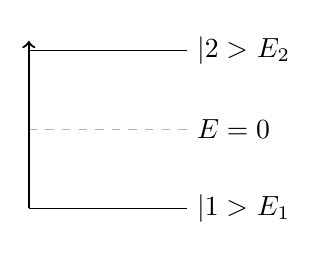
\begin{tikzpicture}
		\tikzstyle{level}=[draw=none,minimum width=2.0cm,minimum height=0.01cm]
		
		\node (A) at (0,-1) [level, label={right:$|1>$ $E_1$}]  {};
		\node (O) at (0,0) [level, label={right:$E=0$}] {};
		\node (B) at (0,1) [level, label={right:$|2>$ $E_2$}] {};
		
		\draw (A.west)--(A.east);
		\draw[dashed, opacity=0.3] (O.west)--(O.east);
		\draw (B.west)--(B.east);
		\draw[thick ,->, label={above left:$E$}] (A.west)--(B.north west);
				
		
		\end{tikzpicture}
		\caption{Átomo de dos niveles}
		\label{fig: two level}
	\end{center}
\end{figure} 

Tomando como referencia a la energía intermedia entre ambos niveles (figura \ref{fig: two level}), podemos escribir a las energías de ambos niveles    como  

\[ \begin{cases}
	E_1=-\frac{\hbar}{2}w_{21}\\
	E_2=\frac{\hbar}{2}w_{21}
\end{cases}
\]

y reemplazando en la ecuación (\ref{eq: h at 1}) ahora el hamiltoniano del átomo se escribe como 

\begin{equation}
	H_{at}=\frac{\hbar}{2}w_{21} [b^{\dagger}_2b_2-b^{\dagger}_1b_1]=\hbar w_{21} \sigma_3
	\label{eq: h at final}
\end{equation}

Donde $\sigma_3$ es la inversión de población.


\subsubsection{El Hamiltoniano del campo electromagnético}

Por otro lado, de la cuantizacion del campo electromagnético, se tiene que 

\begin{equation}
	H_c=\hbar w_{\lambda}(a^{\dagger}_{\lambda}a_{\lambda}+1/2)
	\label{eq: h electro}
\end{equation}


\subsubsection{El Hamiltoniano de interacción}

Por ultimo, si pensamos al átomo de dos niveles como un  dipolo, la interacción del dipolo con el campo electromagnético se puede escribir como 

\begin{equation}
	H_{int}=\frac{1}{2m}(\bar{p}-e\bar{A})^2+V(r)
	\label{eq: h int 1}
\end{equation}


donde puedo escribir el termino $(\bar{p}-e\bar{A})^2$ como 
\[\frac{1}{2m}(\bar{p}-e\bar{A})^2=\frac{1}{2m}(p^2+e^2A^2+e[p,A])-\frac{e}{m}\bar{p}\bar{A}
\]

Escribiendo a $\bar{A}$ en términos del campo cuantizado

\begin{equation}
\bar{A}(\bar{r})=\sum_{\lambda}\sqrt{\frac{\hbar}{2\epsilon w_{\lambda}V}} (a^{\dagger}_{\lambda}e^{i\bar{k}_{\lambda}\bar{r}}+a_{\lambda}e^{-i\bar{k}_{\lambda}\bar{r}})
\end{equation}


\begin{equation}
\bar{E}(\bar{r})=\sum_{\lambda}\sqrt{\frac{\hbar}{2\epsilon w_{\lambda}V}} (a^{\dagger}_{\lambda}e^{i\bar{k}_{\lambda}\bar{r}}+a_{\lambda}e^{-i\bar{k}_{\lambda}\bar{r}})
\end{equation}

Aproximaciones

\begin{itemize}
	\item El termino $\frac{p^2}{2m}$ se puede despreciar argumentando que cada átomo tiene una energía cinética aleatoria, por lo tanto el valor medio de la energía cinética es $0$.
	
	\item El termino $[\bar{p},\bar{A}]=-i\hbar\partial_{q}A=-i\hbar\nabla \cdot A=0 $.
	
	\item El termino $e^2\bar{A}^2=e^2\sum_{\lambda}\alpha^2_{\lambda}((a^{\dagger})^2e^{i2kr}+[a,a^{\dagger}]+(a^2e^{-i2kr})$.
	Los términos con el doble de frecuencia se desprecian por tener poca ganancia%, mientras que el anticonmutador da $0$. neceita un campo muy grande. interacc foton-foton
	
\end{itemize}
\textcolor{red}{terminar esta parte}

por lo tanto, 

\begin{equation}
	H_{int}=-\frac{e}{m}\bar{p}\bar{A}
\end{equation}

.....

\begin{equation}
	H_{int}=-\frac{e}{m}\int \sum_{\lambda j j'}b^{\dagger}_j\varphi^*_j \sqrt{\frac{\hbar}{2\epsilon w_{\lambda}V}}\bar{p} (a^{\dagger}_{\lambda}e^{i\bar{k}_{\lambda}\bar{r}}+a_{\lambda}e^{-i\bar{k}_{\lambda}\bar{r}})b_{j'}\varphi_{j'}
\end{equation}

por lo tanto las integrales se reducen a los elementos de matriz de $\bar{p}$

\begin{equation}
	p_{jj'}=m\dot x{jj'}=m[H,x]_{jj'}=\frac{im}{\hbar}(E_j-E_{j'})x_{jj'}=imw_{jj'}x_{jj'}
\end{equation}

Por lo tanto se obtiene

\begin{equation}
	H_{int}=-i\sum_{\lambda j j'} \sqrt{\frac{\hbar}{2\epsilon w_{jj'}V}}  (a^{\dagger}_{\lambda}e^{i\bar{k}_{\lambda}\bar{r}}+a_{\lambda}e^{-i\bar{k}_{\lambda}\bar{r}})    \int \varphi^*_j ex_{jj'}\varphi_{j'} b^{\dagger}_jb_{j'}
\end{equation}

donde la única integral que queda por hacer ahora es el valor medio de $ex_{jj'}$, el cual no es otra cosa que el momento dipolar clásico.


\begin{equation}
	H_{int}=-i\sum_{\lambda j j'} \sqrt{\frac{\hbar}{2\epsilon w_{jj'}V}}  (a^{\dagger}_{\lambda}e^{i\bar{k}_{\lambda}\bar{r}}+a_{\lambda}e^{-i\bar{k}_{\lambda}\bar{r}})    \langle \mu \rangle_{jj'} b^{\dagger}_jb_{j'}
\end{equation}

Planteando ahora que el sistema tiene solo dos niveles, $j,j'=1;2$

\begin{equation}
	H_{int}=-i\sqrt{ \frac{\hbar w_{21}^2}{2\epsilon V w_{\lambda} } } [....]
\end{equation}

suponiendo que ...

\begin{equation}
	H_{int}=-i\sqrt{ \frac{\hbar w_{21}^2}{2\epsilon V w_{\lambda} } }  [ \langle \mu \rangle_{21}(a^{\dagger}_{\lambda}+a_{\lambda})(b^{\dagger}_2b_{1}) + \langle \mu \rangle_{12} (a^{\dagger}_{\lambda}+a_{\lambda})(b^{\dagger}_1b_{2})  ]
\end{equation}

\[  \langle \mu \rangle_{21}=\langle \mu \rangle_{12}=\langle \mu \rangle   \]

\[\langle \mu \rangle_{11}=\langle \mu \rangle_{22}=0\]

Definiendo a la polarización como :

\begin{equation}
	\begin{cases}
		\sigma^+=b^{\dagger}_2b_{1}\\
		\sigma^-=b^{\dagger}_1b_{2}
	\end{cases}
\end{equation}

$\sigma^+$ representa la transición del estado $|1>$ al estado $|2>$, mientras que $\sigma^-$ representa la transicion del estado $|2>$ al estado $|1>$

\begin{equation}
H_{int}=-i\sqrt{ \frac{\hbar w_{21}^2}{2\epsilon V w_{\lambda} } }   \langle \mu \rangle (a^{\dagger}_{\lambda}+a_{\lambda})(\sigma^+ + \sigma^-) 
\label{eq: h int final}
\end{equation}

\subsubsection{El Hamiltoniano total y la evolución temporal}

Ahora podemos escribir el hamiltoniano total juntando los resultados obtenidos a partir de las ecuaciones (\ref{eq: h int final}), (\ref{eq: h electro}) y (\ref{eq: h at final}).

\begin{equation}
	H=\hbar w_{21} \sigma_3 + \hbar w_{\lambda}(a^{\dagger}_{\lambda}a_{\lambda}+1/2) + -i\sqrt{ \frac{\hbar w_{21}^2}{2\epsilon V w_{\lambda} } }   \langle \mu \rangle (a^{\dagger}_{\lambda}+a_{\lambda})(\sigma^+ + \sigma^-) 
\end{equation}

donde 

\begin{equation}
	\begin{cases}
		\sigma^+=b^{\dagger}_2b_{1}\\
		\sigma^-=b^{\dagger}_1b_{2}\\
		\sigma_3=\frac{1}{2}[b^{\dagger}_2b_2-b^{\dagger}_1b_1]	
	\end{cases}
\end{equation}

aplicando la ecuación de Heinsenberg para la evolución temporal de $\sigma_3$ y $\sigma^+$:

\begin{equation}
	\begin{cases}
		\partial_t \sigma^+=-\frac{i}{\hbar}[\sigma^+,H]\\

		\partial_t \sigma_3=-\frac{i}{\hbar}[\sigma_3,H]	
	\end{cases}
\end{equation}

\begin{equation}
\begin{cases}
[\sigma_3,\sigma^+]=-\sigma^+\\
[\sigma_3,\sigma^-]=-\sigma^-\\
[\sigma^+,\sigma^-]=2\sigma_3\\	
\end{cases}
\end{equation}

que son la evolución temporal de la inversión de población y de la polarización.

\begin{equation}
	\partial_t \sigma_3=-\frac{\langle \mu \rangle }{\hbar}	\sqrt{ \frac{\hbar w_{21}^2}{2\epsilon V w_{\lambda} } } \{ (a^{\dagger}\sigma^+ - a\sigma^- )+a\sigma^+ +a^{\dagger}\sigma^-   \}
\end{equation}


\textcolor{red}{Para la evolucion libre, sin interaccion los operadores evolucionarian de manera tal que }

\begin{equation}
	\begin{cases}
		a(t)=a(0)e^{iw_{\lambda}t}\\
		\sigma^+(t)=\sigma^+(0)e^{iw_0t}
	\end{cases}
\end{equation}

Por lo tanto los terminos con ambos operadores evolucionan aproximadamente de forma que 

\begin{equation}
	\begin{cases}
		a^{\dagger}\sigma^- \approx  e^{-i(w_0-w_{\lambda})t}\\
		a\sigma^+ \approx e^{i(w_0-w_{\lambda})t}\\
		a\sigma^- \approx e^{-i(w_0+w_{\lambda})t}\\
		a^{\dagger}\sigma^+ \approx e^{i(w_0+w_{\lambda})t}
	\end{cases}
\end{equation}

Lo que nos da otro argumento para despreciar los terminos no conservativos cuando $w_{\lambda} \approx w_0$ bajo la aproximacion de \textit{rotating wave}.


\begin{figure}[htc]
	\begin{center}
		
		\begin{tikzpicture}
		\tikzstyle{level}=[draw=none,minimum width=1.5cm,minimum height=0.01cm]
		\tikzstyle{snakeline} = [decorate, decoration={pre length=0.2mm,
			post length=1mm, snake, amplitude=.4mm,
			segment length=2mm}, ->]
		\tikzstyle{connector} = [->]

%%%%%%%%%%%%%%%%%%%%%%%%%%%%%%%%%%%%%%%%%%%%%%%%%%%%%%%%%%%%%%%		
		\node (A1) at (0,-1) [level,label={below: Absorcion} ]  {};
		\node (O1) at (0,0) {};
		\node (B1) at (0,1) [level,label={above:$a^{\dagger}\sigma^+$}] {};
		
		\draw (A1.west)--(A1.east);
		\draw (B1.west)--(B1.east);
		\draw[connector] (A1)--(B1);
		\draw[snakeline] ($(O1)-(1.0cm,0cm)$) -- node[above left] {$\gamma$} ++(O1);
%		\tkzLabelSegment[below=2pt](F,G){Modulador Electro Optico}
%%%%%%%%%%%%%%%%%%%%%%%%%%%%%%%%%%%%%%%%%%%%%%%%%%%%%%%%%%%%%%%			
		\node (A2) at (4,-1) [level,label={below: No conserva E} ]  {};
		\node (O2) at (4,0) {};
		\node (B2) at (4,1) [level, label={above:$a^{\dagger}\sigma^-$}] {};
		
		\draw (A2.west)--(A2.east);
		\draw (B2.west)--(B2.east);
		\draw[connector] (B2)--(A2);
		\draw[snakeline] ($(O2)-(1.0cm,0cm)$) -- node[above left] {$\gamma$} ++(O2);
%%%%%%%%%%%%%%%%%%%%%%%%%%%%%%%%%%%%%%%%%%%%%%%%%%%%%%%%%%%%%%%
		\node (A3) at (8,-1) [level,label={below: No conserva E}]  {};
		\node (O3) at (8,0) {};
		\node (B3) at (8,1) [level, label={above:$a\sigma^+$}] {};
		
		\draw (A3.west)--(A3.east);
		\draw (B3.west)--(B3.east);
		\draw[connector] (A3)--(B3);
		\draw[snakeline] (O3) -- node[above right] {$\gamma$} ++(1.0cm,0cm);
%%%%%%%%%%%%%%%%%%%%%%%%%%%%%%%%%%%%%%%%%%%%%%%%%%%%%%%%%%%%%%%
		\node (A4) at (12,-1) [level,label={below: Emision}, label={right:$|1>$}]  {};
		\node (O4) at (12,0) {};
		\node (B4) at (12,1) [level, label={above:$a\sigma^-$}, label={right:$|2>$}] {};
		
		\draw (A4.west)--(A4.east);
		\draw (B4.west)--(B4.east);
		\draw[connector] (B4)--(A4);
		\draw[snakeline,label={[above right]{$\gamma$}}] (O4) -- node[above right] {$\gamma$} ++(1.0cm,0cm);
		
		
		\end{tikzpicture}
		\caption{Interacciones del átomo de dos niveles}
		\label{fig: interacciones}
	\end{center}
\end{figure} 


\begin{equation}
	\partial_t \sigma_3=-\frac{\langle \mu \rangle }{\hbar}	\sqrt{ \frac{\hbar w_{21}^2}{2\epsilon V w_{\lambda} } } \{ a\sigma^+ + a^{\dagger}\sigma^-   \}
\end{equation}


Para la polarización:

\begin{align}
	\partial_t \sigma_+ & =-\frac{i}{\hbar}[\sigma_+,H]	 \nonumber \\
						& = iw_{21}\sigma^+ - \frac{\langle \mu \rangle }{\hbar} \sqrt{ \frac{\hbar w_{21}^2}{2\epsilon V w_{\lambda} } }    \{ [\sigma^+,a\sigma^+]+[\sigma^+,a^{\dagger}\sigma^-]   \} \nonumber \\
						& =  iw_{21}\sigma^+ - 2 \frac{\langle \mu \rangle }{\hbar} \sqrt{ \frac{\hbar w_{21}^2}{2\epsilon V w_{\lambda} } }   a^{\dagger}\sigma_3
\end{align}



Por otro lado se puede realizar la misma cuenta para $a^{\dagger}$

\begin{align}	
	\partial_t a^{\dagger} &= -\frac{i}{\hbar}[a^{\dagger},H] \nonumber \\
	&= -\frac{i}{\hbar} \{ \hbar w_{\lambda}[a^{\dagger},a^{\dagger}_{\lambda}a_{\lambda}] + -i\sqrt{ \frac{\hbar w_{21}^2}{2\epsilon V w_{\lambda} } }   \langle \mu \rangle (  [a^{\dagger},a^{\dagger}\sigma^-]  +  [a^{\dagger},a\sigma^+]  ) \}     	
\end{align}

Usando las reglas de conmutación y que $ [a^{\dagger},a]=1$

\begin{equation}
	\partial_t a^{\dagger}= -\frac{i}{\hbar} \{ \hbar w_{\lambda}a^{\dagger} + -i\sqrt{ \frac{\hbar w_{21}^2}{2\epsilon V w_{\lambda} } }   \langle \mu \rangle \sigma^+  \}     	
\end{equation}

\begin{equation}
\begin{cases}
	\partial_t a^{\dagger}=  -i w_{\lambda}a^{\dagger} + \sqrt{ \frac{\hbar w_{21}^2}{2\epsilon V w_{\lambda} } }  \frac{\langle \mu \rangle }{\hbar}	 \sigma^+    \\
	\partial_t \sigma_+ =  iw_{21}\sigma^+ - 2 \frac{\langle \mu \rangle }{\hbar} \sqrt{ \frac{\hbar w_{21}^2}{2\epsilon V w_{\lambda} } }   a^{\dagger}\sigma_3\\
	\partial_t \sigma_3=-\frac{\langle \mu \rangle }{\hbar}	\sqrt{ \frac{\hbar w_{21}^2}{2\epsilon V w_{\lambda} } } \{ a\sigma^+ + a^{\dagger}\sigma^-   \}
\end{cases}
\label{eq: quantum rates}
\end{equation}
Definiendo 

\begin{equation}
	\begin{cases}
		\mathcal{P}=\frac{1}{N}\sum_{n=1}^{N}(\sigma^+)_n\\ 
		
		D=\frac{1}{N}\sum_{n=1}^{N}(\sigma_3)_n	
\end{cases}
\end{equation}



Ahora suponemos que el medio interactua con un campo externo coherente de la forma 
\[ E_{ext}=-i \frac{\hbar w_{21}^2}{2\epsilon V w_{\lambda} }  a^{\dagger} e^{-i(kz-wt)}  \]
\textcolor{red}{chequear la cte.}
\[\bar{E}(\bar{r})=\sum_{\lambda}\sqrt{\frac{\hbar}{2\epsilon w_{\lambda}V}} a^{\dagger}_{\lambda}e^{i\bar{k}_{\lambda}\bar{r}}  \]

Por lo tanto puedo escribir a $a$ y $a^{\dagger}$ como :
\begin{equation}
\begin{cases}
\frac{\hbar w_{21}^2}{2\epsilon V w_{\lambda} } a^{\dagger} = i E_{ext} e^{i(kz-wt)}\\
\frac{\hbar w_{21}^2}{2\epsilon V w_{\lambda} }  a = -i E^*_{ext} e^{-i(kz-wt)}\\
\end{cases}
\end{equation}

Remplazando en las ecuaciones (\ref{eq: quantum rates})

\begin{equation}
	\begin{cases}
		\partial_t E_{ext}= -i \hbar w_{\lambda}a^{\dagger} + \sqrt{ \frac{\hbar w_{21}^2}{2\epsilon V w_{\lambda} } }  \frac{\langle \mu \rangle }{\hbar}	 \sigma^+ \\
		\partial_t P =  iw_{21}\sigma^+ - 2 \frac{\langle \mu \rangle }{\hbar} \sqrt{ \frac{\hbar w_{21}^2}{2\epsilon V w_{\lambda} } }   a^{\dagger}\sigma_3\\
		\partial_t D=-\frac{\langle \mu \rangle }{\hbar}	\sqrt{ \frac{\hbar w_{21}^2}{2\epsilon V w_{\lambda} } } \{ a\sigma^+ + a^{\dagger}\sigma^-   \}
	\end{cases}
	\label{eq: quantum clasic rates}
\end{equation}



\textcolor{red}{Ojo que haca hay una aprox}

\textcolor{red}{Preg: le queda complejo con esto}


\textcolor{red}{revisar las constantes y ordenar mejor lo del hamiltoniano de interacción}

	
	\subsection{Metodo semiclasico: Relaciones de Maxwell-bloch}		

		La principal ventaja del metodo semiclasico es que , a diferencia de la deduccion cuantica, es facil proponer la dependencia espacial de las ecuaciones.
		
		Sin embargo, una deduccion completa a partir de una teoria clasica fallaria, entre otras cosas, en describir fenomenos como la emision espontanea, por lo tanto no se podrian deducir dinamicas como la de la lampara comun (sin lasear).
		
		Estos efectos se pueden introducir luego de manera AD HOC. 
		
		\textcolor{red}{chequear lo que puse aca.}
		
		En nuestro caso, con el fin de dar mas claridad a algunas de las aproximaciones hechas que son consideradas de importancia, vamos a deducir la dinamica del campo electrico a partir de las ecuaciones de maxwell clasicas y luego agregarles las ecuaciones de Bloch deducidas a partir de las interacciones cuanticas. 
		
		Ecuaciones de Maxwell:
		
		\begin{equation}
		\begin{cases}
		\bar{\nabla} \times \bar{H} = \bar{J} + \partial_{t} \bar{D}  \\
		\bar{\nabla} \times \bar{E} = -\partial_{t} \bar{B} \\
		\bar{\nabla} \cdot \bar{B}   = 0 \\
		\bar{\nabla} \cdot \bar{D}   = \rho \\
		\end{cases}
		\label{eq: Maxwell}
		\end{equation}  %alinear los iguales.
		
		Suponiendo que el material es lineal, $\bar{D}=\epsilon_0 \bar{E}+\bar{P}$ y $\bar{B}=\mu \bar{H} + \bar{M}$
		
		donde $H$, $M$, ....
		
		y utilizando que $\bar{\nabla} \times (\bar{\nabla} \times \bar{E} )= \bar{\nabla}(\nabla \cdot \bar{E}) - \nabla^2 \bar{E} $
		en $\bar{\nabla} \times (\bar{\nabla} \times \bar{E}) = -\bar{\nabla} \times (\partial_{t} \bar{B})$ y reescribiendo el termino de $\nabla \cdot \bar{E}$ se obtiene 
		
		\[ -\nabla^2 \bar{E} + \nabla (\nabla \cdot (\frac{\bar{D}-\bar{P}}{\epsilon_0}))=-\partial_t (\mu_0 (\bar{\nabla}\times\bar{H} + \bar{\nabla}\times\bar{M} ))  \]
		
		despejando y usando que $\mu_0 \epsilon_0 = \tfrac{1}{c^2}$ se obtiene que 
		
		\begin{equation}
		-\nabla^2 \bar{E} - \frac{1}{c^2} \partial_t \bar{E} = \mu_0 (\partial_t (\bar{\nabla} \times \bar{M})+\partial_t J + \partial^{2}_{t} \bar{P}) + \nabla(\bar{\nabla} \cdot \bar{E})  	
		\end{equation}
		
		Usando como hipótesis que el medio dieléctrico no es magnético ($\rho_l=\jmath_l=0$) .
		Por lo tanto  $\bar{M}=0$, $\bar{j}=0$, $\rho=0$ entonces
		
		\[\bar{D}=\epsilon(r)\bar{E}=\epsilon_0 \epsilon_r(r) \bar{E}\]	
		
		Si el medio es homogéneo , $\bar{\nabla}\cdot \bar{E}=0$, por lo tanto se obtiene la relación de Maxwell-Bloch para un dieléctrico.
		
		
		\begin{equation}
		\nabla^2 \bar{E} - \frac{1}{c^2}\frac{\partial^2 \bar{E}}{\partial t^2}= \mu_0 \frac{\partial^2 \bar{P}}{\partial t^2}
		\label{eq: maxwell-bloch}
		\end{equation}
		
		
		

	
			
				\subsection{Normalizaciones y aproximaciones}
				
				\subsubsection{Campo unidireccional}
				
				Se toma al campo como yendo en dirección positiva en $\hat{z}$ (eje longitudinal del medio), es decir que el ring laser solo funciona en una dirección.
				
				Por lo tanto  $E(r,z,t)=E_x(r,t) e^{i(k_0 z - w_0 t)} + E_y(r,t) e^{i(k_0 z - w_0 t)} $
				
				tomando \[E(r,z,t)=\frac{\hbar \sqrt{ \gamma_{\bot} \gamma_{||} }}{2\mu } \frac{1}{2} [F(r,z,t) e^{i(k_0 z - w_0 t)} + c.c.]  \]
				
				y normalizando $\tau=\gamma_{\bot} t$ , $\eta=\tfrac{z}{L}$ , $v=\frac{c}{L \gamma_{\bot}}$ por lo tanto 
				\[ \partial_t = \gamma_{\bot} \partial_{\tau} \]
				\[ \partial_z = \frac{1}{L} \partial_{\eta}  \]
				
				
				$\delta_{ac}'=\frac{w_a - w_0}{\gamma_{\bot}}$
				donde $w_a$ es la frecuencia de transición atómica, y $w_0$ la frecuencia de la longitud de onda fundamental de la cavidad.
				
				
				\subsubsection{Onda plana}
				
				Suponiendo que dentro del  medio el haz de luz es homogéneo en las direcciones transversales (.. in focus)
				
				\[ \nabla^2 \bar{E} = \nabla^2_{\bot}\bar{E} + \partial^2_z \bar{E} \approx \partial^2_z \bar{E} \]
				
				Por lo tanto 
				\begin{align*}
				\partial^2_z \bar{E} &= \frac{\hbar \sqrt{ \gamma_{\bot} \gamma_{||} }}{2\mu }\frac{1}{2} \{ [\partial^2_z F + 2i k_0 \partial_z F -k_0^2 F]e^{i(k_0 z - w_0 t)} + c.c.  \} \\  
				\partial_t \bar{E} &= \frac{\hbar \sqrt{ \gamma_{\bot} \gamma_{||} }}{2\mu }\frac{1}{2} \{ [\partial_t F - iw_0 F ] e^{i(k_0 z - w_o t)} + c.c. \}  \\
				\partial^2_t \bar{E} &= \frac{\hbar \sqrt{ \gamma_{\bot} \gamma_{||} }}{2\mu }\frac{1}{2} \{ [ \partial^2_t F -2iw_0 \partial_t F -w_0^2  F  ]e^{i(k_0-w_0t)} +c.c. \} 
				\end{align*}
				
				usando que $k_0=\frac{w_0}{c}$ , entonces $(-k_0^2+\frac{w_0^2}{c^2})F=0$
				
				\subsubsection{Variacion lenta de la amplitud}
				
				Para los LASER que es busca modelar, debido a las frecuencias en las que funcionan y a la escala temporal tipica a la que suceden las oscilaciones, se puede realizar la siguiente aproximacion:
				
				\[ \partial^2_t F\ll 2iw_0 \partial_t F
				    \]  
				
				La cual se la llama Varicion lenta de la amplitud. Parte de la validez de la ecuacion se debe a que la frecuencia del campo en los casos de interes suele estar en el rango visible.
				
				Asi como es valido realizar la aproximacion anterior, analogamente se puede realizar la misma aproximacion para la parte espacial. 
				Esto se debe en parte  a que $\bar{k}=w/c$, que en este caso como $\bar{k}=k\bar{z}$ relaciona directamente $k$ con $w$.
				
				
				 \[\partial^2_z F \ll 2ik_0\partial_z F 
				 \] 
				
				
				\[ \partial^2_{z} E - \frac{1}{c^2}\partial^2_{t}\approx  \frac{\hbar \sqrt{ \gamma_{\bot} \gamma_{||} }}{2\mu }\frac{1}{2} {[2ik_0 \partial_z F +2i\frac{w_0}{c^2}\partial_t]e^{i(k_0 z -w_0 t)}+c.c.} 
				\]
				
				De manera similar con $P$, y usando maxwell-bloch:
				
				\begin{equation}
				\begin{cases}
				\partial_{\eta}F+\frac{1}{c/(l\gamma_{\bot})}\partial_{\tau}F= -\frac{\alpha 2 \mu w_0^2}{k_0 \hbar \sqrt{ \gamma_{\bot} \gamma_{||} }} P\\
				\partial_{\tau} P=-{(1+\delta_{ac}')P+FD}\\
				\partial_{\tau}D=-\gamma_{||}\{\frac{1}{2}(F^*P+FP^*)+D-D_0\}
				\end{cases}
				\label{eq: eqs 1}
				\end{equation}  %alinear los iguales.
				
	\subsubsection{Modulacon de la fase: Modulador electro-optico.}
				
				Obs: $I=|E|^2=|E_x|^2+|E_y|^2=I_x+I_y$ porque $E_x\cdot E_y=0$. Es decir que no hay terminos de interferencia entre las dos polarizaciones. Toda la interaccion pasa por los atomos dentro del medio.
				
				Redefiniendo las constantes de la ecuacion \ref{eq: eqs 1}
				
				\begin{equation}
				\begin{cases}
				\frac{c}{l\gamma_{\bot}}\partial_{\eta}F+\partial_{\tau}F= \mu P\\
				\partial_{\tau} P=-{(1+\delta_{ac}')P+FD}\\
				\partial_{\tau}D=-\gamma_{||}\{\frac{1}{2}(F^*P+FP^*)+D-D_0\}
				\end{cases}
				\label{eq: eqs 2}
				\end{equation}  %alinear los iguales.
				
				\begin{figure}[htc]
					\begin{center}
						
						\begin{tikzpicture}
						\coordinate (O) at (-3,-0.5);
						\coordinate (A) at (0,-0.5);
						\coordinate (B) at (0,.5);
						\coordinate (C) at (-3,.5);
						\draw[fill=grey,opacity=.7] (O)--(A)--(B)--(C)--cycle;
						
						\coordinate (OO) at (0,0);
						\coordinate (D) at (4,0);
						\draw[ultra thick, color=red,->] (OO)--(D);
						
						\coordinate (F) at (4,-0.5);
						\coordinate (G) at (5,-0.5);
						\coordinate (H) at (5,.5);
						\coordinate (I) at (4,.5);
						\draw[fill=orange,pattern=north east lines,opacity=.4] (F)--(G)--(H)--(I)--cycle;
						
						\coordinate (J) at (5,0);
						\coordinate (K) at (9,0);
						\draw[ultra thick, color=red,->] (J)--(K);
						
						\tkzLabelSegment[below=2pt](F,G){Modulador Electro Optico}
						\tkzLabelSegment[above=2pt](OO,D){$I$}
						
						\end{tikzpicture}
						\caption{Modulador esquema}
						\label{fig: EOM}
					\end{center}
					
				\end{figure}
				
				
				Antes de pasar por el modulador electro óptico (EOM), $I=I_x+I_y$, luego de pasar por el modulador electro óptico $I=\alpha^2 I_x+\beta^2 I_y$
				
				\begin{equation}
				\begin{bmatrix}
				E_x\\
				E_y
				\end{bmatrix}
				=
				\begin{bmatrix}
				E_{0x}e^{i\phi_x}\\
				E_{0y}e^{i\phi_y}
				\end{bmatrix}
				e^{i(kz-wt)}
				\label{eq: EOM 1}
				\end{equation}
				
				Pensando al \textit{EOM} como una celda de Pockell que se comporta como una placa .... .
				Eligiendo los ejes del EOM, la ecuacion \ref{eq: EOM 1} como
				
				\begin{equation}
				E_{in}=
				\begin{bmatrix}
				E_{x}\\
				E_{y}e^{i\delta_y}
				\end{bmatrix}
				\label{eq: EOM 2}
				\end{equation}
				
				\begin{equation}
				E_{out}=
				\begin{bmatrix}
				E_{x}\\
				E_{y}e^{i(\delta_y + \Delta \phi)}
				\end{bmatrix}
				\label{eq: EOM 3}
				\end{equation}
				
				donde $\Delta \phi $ para el EOM esta dado por 
				
				\begin{equation}
				\Delta \phi = \Delta \phi_0 - \pi \frac{V}{V_{\pi}}
				\end{equation}
				
				donde $V_{\pi}$ es el voltaje que produce una variación en la birrefringencia equivalente a un cambio de fase de $\pi $ .
				
				\[ \Delta \phi_0 =[2\pi(n_e-n_0)\tfrac{L}{\lambda}] \]
				
				donde $n_e$ es el indice extraordinario, y $n_0$ es el indice ordinario. $ L$ es la longitud del cristal y $\lambda $ la longitud de onda en el vacio.
				
				
				\begin{equation}
				E_{out}=
				\begin{bmatrix}
				1 & 0\\
				0 & e^{-i\Delta \phi}
				\end{bmatrix}
				\begin{bmatrix}
				E_{x}\\
				E_{y}e^{i\delta_y }
				\end{bmatrix}
				\label{eq: EOM 4}
				\end{equation}
				
				Por lo tanto, luego de reflejarse en los espejos, los campos quedan descriptos por 
				
				\begin{equation}
				\begin{cases}
				
				E'_x=R E_x\\
				E'_y=R E_y e^{-i(\Delta \phi - \delta_y)}
				\end{cases}
				\end{equation}
				
				calculando ahora el valor de $I'$ se obtiene que , desperdiciando las perdidas, $I'=I$.
				
				\subsection{Condiciones de borde}
				
				
			
				\begin{align}
				F_x(\eta,\tau)|_{\eta=0}&=R F_x(\eta,\tau)|_{\eta=1}\\
				F_y(\eta,\tau)|_{\eta=0}&=R F_y(\eta,\tau)|_{\eta=1} e^{-i\Delta \phi}
				\end{align}
				\label{eq: cc}
			
				
				donde 
				
				\begin{equation}
				\begin{cases}
					F_x(\eta,\tau)=E_x(\eta,\tau)e^{-\eta \ln(R)}\\
					\tilde{P_x}(\eta,\tau)=P_x e^{-\eta \ln(R)}\\			
					F_y(\eta,\tau)=E_y(\eta,\tau)e^{-\eta \ln(R)}e^{i\Delta \phi \eta}\\
					\tilde{P_y}(\eta,\tau)=P_y e^{-\eta \ln(R)}e^{i\Delta \phi \eta}
				\end{cases}
				\end{equation} 			
				
				Reemplazando en las ecuaciones \ref{eq: cc} se obtiene
				\begin{equation}
				E_x(0,\tau)=R E_x(1,\tau)e^{-ln(R)}
				\label{eq: cc2}
				\end{equation}
				
				condición de contorno de ring laser: $E(0,\tau)=E(1,\tau)$
				
		Finalmente se obtienen las ecuaciones que vamos a estudiar:
		
		\[
		\begin{cases}
		\partial_{\tau} E_x=-k E_x + \mu P_x \\
		\partial_{\tau} E_y=-k E_y + \mu P_y + i(\Delta \phi_0 + m.cos(w_{mod}\tau))E_y \\
		\partial_{\tau} P_{x,y}=-(1+i\delta)P_{x,y}+E_{x,y}D \\
		\partial_{\tau} D=-\gamma_{||}(D-D_0+\tfrac{1}{2}(E^*_{x,y}P_{x,y}+E_{x,y}P^*_{x,y})) \\
		\end{cases}
		\label{eq: final eqs 1}
		\]
		
%		
%		with $ E_{x,y}$ and $P_{x,y}$  $\in \mathbb{C}$
%		
		donde 
		\begin{itemize}
			\item $k$ es la razón entre el ancho de la cavidad (cavity linewidth) y el ancho espectral (atomic linewidth).
			\item $\mu$ es la ..
			\item $\delta $  es un parámetro de sintonizacion (detuning) de la cavidad.
			\item $\Delta \phi_0 $ es el  \textit{offset} de la modulación . La correlación física de $\Delta \phi_0 $ es la birrefringencia del medio, sumada al cambio de fase inducido por el modulador electro óptico .
			\item $m$ es la amplitud de la modulación . Físicamente ..
			\item $D_0$ 
			\item $\tau$ es el tiempo normalizado.
			\item $\gamma_{||}$ es taza de relajación para la inversión de población (relaxation rate) .
			\item $\gamma_{\bot}$ es ancho espectral (atomic lindewidth) .
		\end{itemize}
		
		
		Escribiendo los campos como parte real e imaginaria:
		
		\[
		\begin{cases}
		\partial_{\tau} Re(E_x)=-k Re(E_x) + \mu Re(P_x) \\
		\partial_{\tau} Im(E_x)=-k Im(E_x) + \mu Im(P_x) \\
		\partial_{\tau} Re(E_y)=-k Re(E_y) + \mu Re(P_y) -(\Delta \phi_0 + m.cos(w_{mod}.\tau)).Im(E_y) \\
		\partial_{\tau} Im(E_y)=-k Im(E_y) + \mu Im(P_y) + (\Delta \phi_0 + m.cos(w_{mod}.\tau)).Re(E_y) \\
		\partial_{\tau} Re(P_{x,y})=-(Re(P_{x,y})-Im(P_{x,y})\delta)+Re(E_{x,y}).D \\
		\partial_{\tau} Im(P_{x,y})=-(Im(P_{x,y})+Re(P_{x,y})\delta)+Im(E_{x,y}).D \\
		\partial_{\tau} D=-\gamma_{||}(D-D_0+(Re(E_{x,y})Re(P_{x,y})+Im(E_{x,y})Im(P_{x,y}))) \\
		\end{cases}
		\]
		
		\begin{lstlisting}
		def mb(y, t,k,mu,Dphi0,d,g,D0,m,wf):
		""" y[0],y[1] campo electrico en x. y[2],y[3] campo electrico en y, y[4],y[5]  polarizacion en x, y[6],y[7]  polarizacion en y, y[8] poblacion. """
		dfxr=-k*y[0]+mu*y[4]
		dfxi=-k*y[1]+mu*y[5]
		dfyr=-k*y[2]+mu*y[6]-y[3]*(Dphi0+m*np.cos(wf*t))
		dfyi=-k*y[3]+mu*y[7]+y[2]*(Dphi0+m*np.cos(wf*t))
		drxr=-(1*y[4]-d*y[5])+y[0]*y[8]
		drxi=-(1*y[5]+d*y[4])+y[1]*y[8]
		dryr=-(1*y[6]-d*y[7])+y[2]*y[8]
		dryi=-(1*y[7]+d*y[6])+y[3]*y[8]
		ddelta=-g*(y[8]-D0+(y[0]*y[4]+y[1]*y[5]+y[2]*y[6]+y[3]*y[7]))
		return [dfxr,dfxi,dfyr,dfyi,drxr,drxi,dryr,dryi,ddelta]
		\end{lstlisting}
		
		Normalizations made: 
		$\tau= \gamma_{\bot}.t$, $k=\tfrac{\bar{k}}{\gamma_{\bot}}$,  $\gamma_{\parallel}=\tfrac{\bar{\gamma_{\parallel}}}{\gamma_{\bot}}$, $\eta=\tfrac{z}{L}$, $\delta'_{ac}=\tfrac{w_a-w_0}{\gamma_{\bot}}$
		
		
		Aproximations: 
		
		1-$k,\gamma_{\parallel}<<\gamma_{\bot}$   -- Homogenously broadened laser linewidth $ \nabla^2 E-\frac{1}{c^2}\partial^2_{t}E=\alpha \partial^2_{t}E$
		
		2-Plane wave: $\nabla^2_{\bot}=0$
		
		3-Two level medium
		
		4-Slowly varying amplitud
		
		5-Unidirectional field
		
		6-Rotating wave approx $\partial_{t^2}<<\partial_t$
		
		7-Single longitudinal mode
		
		8-$g'->0$, $R_0->1$  -- Uniform field limit
		
		9-$m$,$w_{mod}<<1$, $w_{mod}<<\gamma_{\bot}$ % ..chequear..
	
	
\section{Elección de parámetros del sistema}

	Para este estudio se fijaron los parámetros físicos del sistema de manera que el estudio se concentra en la evolución del sistema al variar los parámetros de modulación, dejando fijo los demás parámetros del láser.
	
	Los parámetros utilizados a lo largo del estudio son :
	\begin{itemize}
		\item $\gamma_{||}=2,5 .10^{-4}$
		\item $k=0,09$Khz
		\item $\mu=2.5 .10^{-5}$
		\item $D_0=7200$
		\item $\delta=1$
	\end{itemize}
	
	donde $k$, $mu$ y  $\gamma_{||}$ fueron elegidos basados en los valores usuales para el láser modelado.
	$D_0$ es fijado pidiendo que la constante $A=\frac{D_0 \mu}{k}=2$, y el valor de $\delta$ es elegido de manera tal que los efectos no lineales sean mas notorios. Para esto se utiliza un valor de $\delta$ que aleje al sistema del máximo de la campana de ganancia ($\delta=0$).
	
	Para este sistema, la frecuencia de resonancia esta determinada por la ecuación 
	
	\[ \Omega=\sqrt{k \gamma_{||} (\frac{D_0 \mu}{k} -1)}=\sqrt{k \gamma_{||} (A -1)}=\sqrt{k \gamma_{||}}=473.34 Khz\]
	
	A continuación se muestran algunas dinámicas del sistema en ausencia de modulación ($m=0$, $\Delta \phi_0 = 0$)
	
%	\textcolor{red}{poner ejemplos sin modulación. }
%		
%		
%	Mientras que a continuación se compara la dinámica del modulo del campo eléctrico para un caso en el cual $\delta =0$ y otro en el que $\delta = 1$
%		
	\begin{minipage}{0.5\textwidth}
		\begin{center}
			\includegraphics[width= \linewidth]{../Python/casos interesantes/comparison no mod short time.png}
		\end{center}
	\end{minipage}
	\begin{minipage}{0.5\textwidth}
		\begin{center}
			\includegraphics[width= \linewidth]{../Python/casos interesantes/comparison no mod long time.png}
		\end{center}
	\end{minipage}
	
	\textcolor{red}{cambiar labels}

	Mientras que a continuación se compara la dinámica del modulo del campo eléctrico para un caso en el cual $\delta =0$ y otro en el que $\delta = 1$


	\textcolor{red}{Poner comparación con y sin $\delta =1 $ }


	En la figura \ref{fig: ci simetrica} se muestra como a partir de una condición inicial simétrica en x e y, el sistema evoluciona manteniendo la simetría, como es esperable.
	\begin{center}
		\includegraphics[width= 0.6\linewidth]{../Python/Imagenes especiales para la tesis/m=0, simetr.png}
		\captionof{figure}{Evolución del sistema sin modulación a partir de la condición inicial simétrica: $E=(1+i1,1+i1)$ ,$ P=(60+i60,60+i60)$, $D=6000$}
		\label{fig: ci simetrica}
	\end{center}
	
%		\begin{center}
%			\includegraphics[width= 0.6\linewidth]{../Python/integ directa/Results/2016_7_26-19.34.48-E_intensitys.png}
%			\captionof{figure}{Evolución del sistema sin modulación a partir de la condición inicial simétrica: $E=(5+i5,5+i5)$ ,$ P=(3000+i3000,3000+i3000)$, $D=6000$}
%			\label{ci simetrica 2}
%		\end{center}
%	
	
	\begin{center}
		\includegraphics[width= 0.6\linewidth]{../Python/Imagenes especiales para la tesis/m=0, asimetr.png}
		\captionof{figure}{Evolución del sistema sin modulación a partir de la condición inicial asimétrica: $E=(2+i2,1+i1)$ ,$ P=(100+i100,60+i60)$, $D=6000$}
	\end{center}
		
		
	Luego se utilizaran los valores finales de este resultado como condición inicial para intentar encontrar otros casos con dinámica 'activa' en ambos campos.	
%	\begin{center}
%		\includegraphics[width= 0.5\linewidth]{../Python/integ directa/Results/casos interesantes/sin modulacion/2016_6_2-17.4.17-E_intensitys.png}
%	\end{center}
	
	Una vez que el sistema se encuentra modulado, se espera que para $\delta=0$ el sistema responda con el doble del periodo de la modulación, mientras que con $\delta\neq 0$ el sistema...  .
	%mejorar esta parte.
	
		\textcolor{red}{Poner figuras con los periodos de ambos casos. }
%	\begin{center}
%		\includegraphics[width= 0.4\linewidth]{../Python/casos interesantes/comparison no mod long time.png}
%	\end{center}
	
	
%	\begin{center}
%		\includegraphics[width= 0.4\linewidth]{../Python/casos interesantes/comparison no mod long time.png}
%	\end{center}



	
	\chapter{Ruptura de simetría y decaimiento de $|E_x|$}
	
	\section{Intensidad y fase }
	
		\subsection{Intensidades}
			
			Para la situaciones en las que decae el campo en la direccion $X$, si no se tiene en cuenta toda la dinamica en esa direccion, se intenta reescribir el termino de en $y$ para la intensidad y la fase.
			
			Definiendo $I_y=Re(E_y)^2+Im(E_y)^2$, y recordando que 
			\[
			\begin{cases}
			\partial_{\tau} Re(E_y)=-k Re(E_y) + \mu Re(P_y) -(\Delta \phi_0 + m.cos(w_{mod}.\tau)).Im(E_y) \\
			\partial_{\tau} Im(E_y)=-k Im(E_y) + \mu Im(P_y) + (\Delta \phi_0 + m.cos(w_{mod}.\tau)).Re(E_y) \\
			\end{cases}
			\]
			
			$\partial_{\tau}I_y=2 Re(E_y)\partial_{\tau}Re(E_y)+2 Im(E_y)\partial_{\tau}Im(E_y)=E_y^*\partial_{\tau}E_y+E_y\partial_{\tau}E_y^*$
			
			por lo tanto queda que 
			
			$\partial_{\tau}I_y=2 [Re(E_y)(-k Re(E_y) + \mu Re(P_y) - \Delta \phi.Im(E_y))+ Im(E_y)(-k Im(E_y) + \mu Im(P_y) + \Delta \phi .Re(E_y))$] 
			
			con lo cual se anulan los términos que tiene la modulación de manera explicita. Reescribiendo un poco la ecuación, se obtiene
			
			\begin{equation}
			\partial_{\tau}I_y=2[-k I_y +\tfrac{1}{2}\mu[E^*_yP_y+E_yP^*_y]   ] 		
			\end{equation}
			
			
			Dado que la modulación se anula, el mismo procedimiento se puede realizar para la intensidad en x y la intensidad total.
			
			\begin{align}
			\partial_{\tau}I_x &= 2[-k I_x +\tfrac{1}{2}\mu[E^*_xP_x+E_xP^*_x] ]  \\
			\partial_{\tau}I &= 2[-k I +\tfrac{1}{2}\mu[E^*_xP_x+E_xP^*_x+E^*_yP_y+E_yP^*_y]]
			\end{align}
			
		\subsection{Fase}
			
			Siendo que para un numero complejo $Z$, $\psi=\arctan(\frac{Im(z)}{Re(z)})$
			
			\[  \psi_y= \arctan(\frac{Im(E_y)}{Re(E_y)}) \]
			
			por  lo tanto , notando $Im(E_y)=E_{yi}$, $Re(E_y)=E_{yr}$ y $\Delta \phi=\Delta \phi_0 + m.cos(w_{mod}.\tau) $ :
			
			\begin{align}
			\partial_{\tau}\psi_y  &= \frac{1}{ 1+\frac{ E^2_{yi} }{ E^2_{yr} } }\frac{ E_{yr} \partial_{\tau}( E_{yi} ) - E_{yi} \partial_{\tau}( E_{yr} ) }{ E^2_{yr} } \\ 
			&= \frac{ E_{yr} ( -kE_{yi}+\mu P_{yi}+\Delta \phi E_{yr} ) -  E_{yi} ( -kE_{yr}+\mu P_{yr}-\Delta \phi E_{yi} ) }{ I_y } \\
			&= \frac{ \mu ( P_{yi} E_{yr} - P_{yr} E_{yi} ) }{ I_y } + \Delta \phi	
			\end{align}
			
			Llamativamente, queda de manera explicita la dependencia con la modulación.
			
			Haciendo lo mismo en $x$, las ecuaciones de los campos eléctricos se pueden reescribir como :
			\begin{equation}
			\begin{cases}
			\partial_{\tau}I_y=2[-k I_y +\tfrac{1}{2}\mu[E^*_yP_y+E_yP^*_y]   ] \\
			\partial_{\tau}I_x=2[-k I_x +\tfrac{1}{2}\mu[E^*_xP_x+E_xP^*_x]   ]	\\	
			\partial_{\tau}\psi_y  = \frac{ \mu ( P_{yi} E_{yr} - P_{yr} E_{yi} ) }{ I_y } + \Delta \phi \\
			\partial_{\tau}\psi_x  = \frac{\mu(P_{xi}E_{xr}-P_{xr}E_{xi})}{I_x}
			\end{cases}
			\label{eq: int y fases}
			\end{equation}
			
			
			%		\subsubsection{Eliminación adiabatica}
			%		
			%		Si se supone que la polarizacion es proporcional a los campos electricos respectivos, osea $P_{x,y} = \alpha E_{x,y}$, entonces 
			%		
			%		\[ 
			%			\begin{cases}
			%				\partial_{\tau}I^2_y=2[-k I^2_y +\tfrac{1}{2}\mu \alpha I^2_y ] \\  
			%				\partial_{\tau}I^2_x=2[-k I^2_x +\tfrac{1}{2}\mu \alpha I^2_x ]\\
			%				\partial_{\tau}\psi_y  = \Delta \phi\\
			%				\partial_{\tau}\psi_x  = 0
			%			\end{cases}
			%		\]
			
			
			Finalmente, para la polarización del haz.
			
			$\Psi=\arctan(\frac{E_{yr} }{E_{xr} })$
			
			\begin{equation}
			\partial_{\tau}\Psi  = \frac{\mu(P_{yr}E_{xr}-P_{xr}E_{yr})-\Delta \phi E_{xr}E_{yr}}{E^2_{yr}+E^2_{xr}}
			\end{equation}
			
			
		
		%		por ultimo, como $I=\rho^2$, entonces $\partial_{\tau}I=2 \partial_{\tau}\rho$
		%		
		%		\[
		%		\begin{cases}
		%		\partial_{\tau} I_x=2[-k \rho_x + \alpha \mu\rho_x D] \\
		%		\partial_{\tau} \varphi_x=-\alpha \mu \tilde{\delta} D +\tilde{\delta w}\
		%		\partial_{\tau} I_y=2[-k \rho_y + \alpha \mu\rho_y D] \\
		%		\partial_{\tau} \varphi_y=-\alpha \mu \tilde{\delta} D +\tilde{\delta w}+\Delta \phi \\
		%		\partial_{\tau} D=-\gamma_{||}(D-D_0+\alpha D I) \\
		%		\end{cases}
		%		\]
		%		
	
	\section{Ruptura de simetría}
		
		Durante las simulaciones se observo que prevalecen los casos en los que el campo $E_x$ decae y la única dinámica significativa para en el eje $y$.
		
		Para estudiar esto , basándonos en los resultados obtenidos reescribiendo los campos eléctricos para la intensidad y la fase \ref{eq: int y fases}, se procedió a integrar al sistema partiendo de una condición inicial simetrica $E=(1+i1,1+i1)$ ,$ P=(300+i300,300+i300)$, $D=6000$ para el sistema sin modulación ($\Delta \phi_0=0$, $m=0$) como se muestra en la figura \ref{fig: ci simetrica2} y luego haciendo lo mismo para el sistema con $\Delta \phi_0=0.01$ (figura \ref{label}) y $\Delta \phi_0=-0.01$ (figura \ref{label}).
		
		Se eligieron estos valores ya que son comparables con los valores utilizados para el parámetro $m$ .
		
		\begin{figure}[htc]
			
			\includegraphics[width= .7\linewidth]{../Python/integ directa/Results/2016_8_10-15.4.54-E_intensitys.png}
			\caption{Evolución del sistema para una condición inicial simetrica $E=(1+i1,1+i1)$ ,$ P=(300+i300,300+i300)$, $D=6000$ para el sistema sin modulación ($\Delta \phi_0=0$, $m=0$)}
			\label{fig: ci simetrica2}
		\end{figure}
		
		\begin{figure}[htc]
			\includegraphics[width= .5\linewidth]{../Python/integ directa/Results/2016_8_10-15.22.13-E_intensitys.png}
			\caption{Evolución del sistema para una condición inicial simétrica $E=(1+i1,1+i1)$ ,$ P=(300+i300,300+i300)$, $D=6000$ para el sistema con ($\Delta \phi_0=0.01$ y  $m=0$}
			\label{fig: ci delta phi 0.01}
		\end{figure}
		\begin{figure}[htc]
			\includegraphics[width= .5\linewidth]{../Python/integ directa/Results/2016_8_10-15.19.0-E_intensitys.png}
			\caption{Evolución del sistema para una condición inicial simétrica $E=(1+i1,1+i1)$ ,$ P=(300+i300,300+i300)$, $D=6000$ para el sistema con $\Delta \phi_0=-0.01$ y $m=0$}
			\label{fig: ci delta phi -0.01}
		\end{figure}
		
		Como se puede observar en este el signo de $\Delta \phi_0$ causa una ruptura de simetría que provoca el decaimiento exponencial de uno de los dos campos.
		
		Esto se puede empezar a entender a partir de los resultados obtenidos de la eliminación abdicativa \ref{eq: elim adiabatica}, en los cuales que muestra que la modulación afecta directamente a la fase $\varphi_y$. Esto implicaría que afecta la ganancia que tiene este mismo campo. Por lo tanto, si tiene una ganancia mayor a la del campo en el eje $x$, esta diferencia provocaría que la influencia de la población en este campo crezca exponencialmente , de manera equivalente, la población tiene una influencia que decae exponencialmente en el campo con menor ganancia.
		
		Esto se debe a que para un valor constante de población en el medio, se puede pensar que la misma es un recurso constante del cual los campos subsisten para poder mantenerse. Lo que puede entenderse como una especie de  'competencia'.
		
		\textcolor{red}{Escribir mejor esto, poner algún gráfico que lo esclarezca.}	
		
		
		\begin{center}
			\includegraphics[width= 0.6\linewidth]{../Python/integ directa/Results/2016_7_27-13.38.21-E_intensitys.png}
			\captionof{figure}{Evolución del sistema sin modulación a partir de la condición inicial asimétrica: $E=(1+i1,1+i1)$ ,$ P=(300+i300,300+i300)$, $D=6000$}
		\end{center}
		
		
		
		\begin{center}
			\includegraphics[width= 0.6\linewidth]{../Python/integ directa/Results/2016_7_27-13.13.55-E_intensitys.png}
			\captionof{figure}{Evolución del sistema sin modulación a partir de la condición inicial asimétrica:$E=(1+i1,1+i1)$ ,$ P=(300+i300,300+i300)$, $D=6000$}
		\end{center}
		
		
		\subsection{Casos con modulación dependiente del tiempo}
		
			En el estudio realizado se observo que con $m=0.02$, para valores de frecuencia mayores a $121.76 $Khz no se pudieron encontrar condiciones iniciales que terminen en una órbita estable en la cual el campo el modulo del campo eléctrico en la dirección $x$ ($|E_x|$) no decae con el tiempo como se muestra en la figura ?????.
			
			
			\begin{minipage}{0.7\textwidth}
				
				\centering
				\includegraphics[width= 1\linewidth]{../Python/integ directa/Results/2016_5_9-18.50.39-E_intensitys.png}
				
			\end{minipage}
			
			\begin{minipage}{0.5\textwidth}
				
				\centering
				\includegraphics[width= 1\linewidth]{../Python/integ directa/Results/2016_5_9-18.38.9-Ex_vs_Ey.png}
				%\caption{Set joke}
				%	\label{fig:erise}
				
			\end{minipage}
			\begin{minipage}{0.5\textwidth}
				
				\centering
				\includegraphics[width= 1\linewidth]{../Python/integ directa/Results/2016_5_9-18.38.9-E_vs_population.png}
				%\caption{Set joke}
				%	\label{fig:erise}
				
			\end{minipage}
			
			
			
			\begin{minipage}{0.6\textwidth}
				
				\centering
				\includegraphics[width= 1\linewidth]{../Python/integ directa/Results/2016_5_9-23.47.40-E_intensitys.png}
				%\caption{Set joke}
				%	\label{fig:erise}
				
			\end{minipage}
			
			\begin{minipage}{0.5\textwidth}
				
				\centering
				\includegraphics[width= 1\linewidth]{../Python/integ directa/Results/2016_5_9-23.47.42-Ex_vs_Ey.png}
				%\caption{Set joke}
				%	\label{fig:erise}
				
			\end{minipage}
			\begin{minipage}{0.5\textwidth}
				
				\centering
				\includegraphics[width= 1\linewidth]{../Python/integ directa/Results/2016_5_9-23.47.42-E_vs_population.png}
				%\caption{Set joke}
				%	\label{fig:erise}
				
			\end{minipage}
			
			Llama la atención que para frecuencias muy bajas, los módulos de los campos oscilan parece oscilar 'tomándose turnos' de actividad, durante los cuales la polarización de haz es lineal, a diferencia de lo que puede ser una polarización circular en al cual el modulo de los campos complejos se mantiene constante.
			
			%	
			%	Mientras que para valores mas bajos de la frecuencia, el sistema pasa por una bifurcación ????? a partir de la cual ambos campos muestran una dinamica .
			
			Mientras que para valores mas bajos de la frecuencia se observa que para algunas condiciones iniciales ninguno de los campos decae .
			
			\begin{minipage}{0.5\textwidth}
				
				\centering
				\includegraphics[width= 1\linewidth]{../Python/integ directa/Results/2016_5_9-19.6.24-E_intensitys.png}
				%\caption{Set joke}
				%	\label{fig:erise}
				
			\end{minipage}
			\begin{minipage}{0.5\textwidth}
				
				\centering
				\includegraphics[width= 1\linewidth]{../Python/integ directa/Results/2016_5_9-19.6.25-E_vs_population.png}
				%\caption{Set joke}
				%	\label{fig:erise}
				
			\end{minipage}
		
		
		
	\section{Multiestabilidad}
		\textcolor{red}{ahora estoy pasando estos resultados a donde están los mapas. Tengo que modificarlo.}
		
		Como ejemplo de un caso claro de multiestabilidad, a continuación se muestran dos evoluciones temporales del modulo del campo eléctrico comparadas con la modulación. 
		En ambos casos se utilizaron los mismos parámetros, pero distintas condiciones iniciales.
		
		\subsection{$m=0.02$, $w=237.3$Khz}
		\begin{minipage}{0.5\textwidth}
			
			\centering
			\includegraphics[width= 1\linewidth]{../Python/integ directa/Results/2016_5_17-15.33.6-comparison.png}
			%\caption{Set joke}
			%	\label{fig:erise}
			
		\end{minipage}
		\begin{minipage}{0.5\textwidth}
			
			\centering
			\includegraphics[width= 1\linewidth]{../Python/integ directa/Results/2016_5_17-15.33.8-E_vs_population.png}
			%\caption{Set joke}
			%	\label{fig:erise}
			
		\end{minipage}
		
		
		
		\begin{minipage}{0.5\textwidth}
			
			\centering
			\includegraphics[width= 1\linewidth]{../Python/integ directa/Results/2016_5_17-15.18.58-comparison.png}
			
		\end{minipage}
		\begin{minipage}{0.5\textwidth}
			
			\centering
			\includegraphics[width= 1\linewidth]{../Python/integ directa/Results/2016_5_17-15.19.0-E_vs_population.png}
			%\caption{Set joke}
			%	\label{fig:erise}
			
		\end{minipage}
		
		
		\subsection{$m=0.02$, $w=100$Khz}
		
		Se muestran tres órbitas estables para $m=0.02$, $w=100$Khz.
		
		\begin{minipage}{0.33\textwidth}
			\centering
			\includegraphics[width= 1\linewidth]{../Python/integ directa/Results/multiestability/2016_6_1-22.53.21-color_phase_E_vs_pop.png}
			%\caption{Set joke}
			%	\label{fig:erise}
			
		\end{minipage}
		\begin{minipage}{0.33\textwidth}
			
			\centering
			\includegraphics[width= 1\linewidth]{../Python/integ directa/Results/multiestability/2016_6_1-23.0.5-color_phase_E_vs_pop.png}
			
		\end{minipage}
		\begin{minipage}{0.33\textwidth}
			
			\centering
			\includegraphics[width= 1\linewidth]{../Python/integ directa/Results/multiestability/2016_6_1-22.57.58-color_phase_E_vs_pop.png}
			
		\end{minipage}
		
		
		De las mimas, solo la ultima presenta dinámica no nula en ambas direcciones del campo electrico.
		
		\begin{minipage}{0.5\textwidth}
			
			\centering
			\includegraphics[width= 1\linewidth]{../Python/integ directa/Results/multiestability/2016_6_1-22.58.1-E_intensitys.png}
			%\caption{Set joke}
			%	\label{fig:erise}
			
		\end{minipage}

		
	\chapter{Mapas}

	\section{Barridos en $m$}
	\textcolor{red}{tengo que cambiar las labels del eje y}
	
		\subsection{Mapa de un barrido en el parámetro $m$, con $\Delta \phi_0 = 0 $ y $w=500$Khz}
		
			\begin{center}
				\includegraphics[width= 0.6\linewidth]{../Python/swype m max/swype_m_max/Results/2016_7_24-13.12.20-Max_vs_m (w=500.0, m=(0.0 - 0.08)).png}
				\captionof{figure}{De menor a mayor}
				\label{fig: mapa m 500 }
			\end{center}
			
			
			\begin{center}
				\includegraphics[width= 0.6\linewidth]{../Python/swype m max/swype_m_max/Results/2016_7_28-17.42.7-compare_Max_vs_m-1.png}
				\captionof{figure}{Otros atractores}
				\label{fig: mapa m 500 colores}
			\end{center}
			
			
		\subsection{Mapa de un barrido en el parámetro $m$, con $\Delta \phi_0 = 0 $ y $w=473.34$Khz}
		
			\begin{center}
				\includegraphics[width= 0.6\linewidth]{../Python/swype m max/swype_m_max/Results/2016_7_24-0.45.12-Max_vs_m (w=473.34, m=(0.0 - 0.08)).png}
				\captionof{figure}{Histeresis}
				\label{fig: mapa m 379 histeresis}
			\end{center}
			
		
%		\subsubsection{Mapa de un barrido en el parámetro $m$, con $\Delta \phi_0 = 0 $ y $w=420$Khz}
%			
%			\begin{center}
%				\includegraphics[width= 0.6\linewidth]{../Python/swype m max/swype_m_max/Results/2016_7_23-5.49.19-Max_vs_m (w=420.0, m=(0.0 - 0.02695)).png}
%				\captionof{figure}{???}
%				\label{fig: mapa m 420}
%			\end{center}		
%			
%			\begin{center}
%				\includegraphics[width= 0.6\linewidth]{../Python/swype m max/swype_m_max/Results/2016_7_23-5.35.47-Max_vs_m (w=420.0, m=(0.0 - 0.02695))-2.png}
%				\captionof{figure}{zoom}
%				\label{fig: mapa m 420 zoom}
%			\end{center}		
%	
%		
%		\subsubsection{Mapa de un barrido en el parámetro $m$, con $\Delta \phi_0 = 0 $ y $w=400$Khz}
%		
%			\begin{center}
%				\includegraphics[width= 0.6\linewidth]{../Python/swype m max/swype_m_max/Results/2016_7_23-8.46.53-Max_vs_m (w=400.0, m=(0.0 - 0.1)).png}
%				\captionof{figure}{????????}
%				\label{fig: mapa m 400 }
%			\end{center}
%			
	
		\subsection{Mapa de un barrido en el parámetro $m$, con $\Delta \phi_0 =0 $ y $w=379$Khz}
		
			Mapa utilizando los máximos del modulo del campo eléctrico :
			
			\begin{center}
				\includegraphics[width= 0.6\linewidth]{../Python/swype m max/swype_m_max/Results/2016_5_22-17.35.3-Max_vs_m (w=379.0, m=(0.01 - 0.036397)).png}
				\captionof{figure}{Barrido del parámetro $m$ para $w=379$kHz}
				\label{fig: mapa m 379}
			\end{center}
			
			Mismo mapa, utilizando una sección estroboscopica del modulo del campo eléctrico.
			Para la sección estroboscopica se toma un el valor del modulo del campo eléctrico para cada máximo de la modulación .
	%				\textcolor{red}{Pone barrido con mismos limites que el otro caso, y en ambos sentidos.}
				
			\begin{center}
				\includegraphics[width= 0.8\linewidth]{../Python/swype m max/swype_m_max/Results/2016_7_31-17.14.7-compare_Max_vs_m.png}
				\captionof{figure}{Barrido del parámetro $m$ para $w=379$kHz}
				\label{fig: mapa m 379 colores}
			\end{center}
					
			\begin{center}
				\includegraphics[width= 0.5\linewidth]{../Python/swype m stroboscopic/Results/2016_5_31-16.45.26-both-strobo_vs_m-2.png}
				\captionof{figure}{Mapa estroboscopico del mismo barrido que en la figura \ref{fig: mapa m 379}. En azul se muestra el barrido creciente, y en rojo el decreciente.}
				\label{fig: swype m 379 strobo histeresis}
				\textcolor{red}{tengo que arreglar esta figura}
			\end{center}
			
			En la figura \ref{fig: mapa m 379 histeresis} se muestra en negro un barrido creciente en $m$, y en rojo un barrido decreciente.
			Se observa la presencia de histeresis.
			
			\begin{center}
				\includegraphics[width= 0.6\linewidth]{../Python/swype m max/swype_m_max/Results/figure_5.png}
				\captionof{figure}{Histeresis}
				\label{fig: mapa m 379 histeresis}
			\end{center}
					
%	\subsubsection{Mapa de un barrido en el parámetro $m$, con $\Delta \phi_0 = 10^{-5} $ y $w=379$Khz}	
			\textcolor{red}{Poner barrido con delta phi 0 }
%			 
		\subsection{Mapa de un barrido en el parámetro $m$, con $\Delta \phi_0 = 0 $ y $w=120$Khz}
		
		Se realizaron barridos del parámetro $m$ para $w=120$kHz , ya que para estas frecuencias se obtuvieron resultados con dinámicas no nulas en ambos campos.
		Para obtener los resultados con ambos campos se empezó a integrar desde  $m=0$ con una condición inicial simétrica como la que se muestra en la figura \ref{fig: ci simetrica}. 
		
			\begin{center}
				\includegraphics[width= 0.6\linewidth]{../Python/swype m max/swype_m_max/Results/2016_7_26-19.12.45-compare_Max_vs_m.png}
				\captionof{figure}{Resultados obtenidos para los barrido con $w_{mod}=120$kHz. En rojo se muestran los resultados obtenidos a partir de una condicion inicial simetrica. En azul se muestra los resultados obtenidos a partir de un barrido decreciente empezando desde las soluciones caoticas para $m>0.5$}
				\label{fig: mapa m 120}
			\end{center}		
		\textcolor{red}{poner mas resultados de este mapa}
		
		Se observa que para valores mayores a $m=0.44$ el sistema vuelve a tener soluciones con decaimiento en el campo electrico en la dirección $x$.		
				
				
	\section{Barrido en $w$}
	
	
	
	
	\subsection{Mapa de un barrido en el parámetro $w$, $m=0.015$ y $\Delta \phi_0=0$}			 		
	
	\begin{figure}[htp]
		\begin{center}
			\includegraphics[width= .48\linewidth]{../Python/swype w max/Results/2016_7_8-19.23.57-Maxintensity_vs_w (m= 0.015, w=( 500.0 - 100.0 )).png}
			\includegraphics[width= .48\linewidth]{../Python/swype w max/Results/2016_7_10-9.52.3-Maxintensity_vs_w (m= 0.015, w=( 100.0 - 500.05 )).png}	
		\end{center}
		\caption{Barrido detallado de mayor a menor(en negro) y de menor a mayor(en azul) conservando la fase de la solucion anterior .}
	\end{figure}	
	
	
		\subsection{Mapa de un barrido en el parámetro $w$, $m=0.0187$ y $\Delta \phi_0=0$}			 
		
			\begin{figure}[H]
				\begin{center}
					\includegraphics[width= .8\linewidth]{../Python/swype w max/Results/2016_7_20-11.59.15-Maxintensity_vs_w (m= 0.0187, w=( 500.0 - 248.15 )).png}
				\end{center}
				\caption{Barrido detallado de mayor a menor.}
			\end{figure}	
			
			
			\begin{figure}[htp]
				\begin{center}
					\includegraphics[width= .5\linewidth]{../Python/integ directa/Results/multiestability crisi/2016_7_20-3.52.17-color_phase_E_vs_pop.png}
				\end{center}
				\caption{Soluciones obtenidas para $w=499.25$kHz. Para valores de $m$ mayores a $1.975$ no se encontraron este tipo de soluciones.}
			\end{figure}		
			\todo{hacer un barrido en m para esta frecuencia a ver hasta donde llegan.}
		
		
		
		\subsection{Mapa de un barrido en el parámetro $w$, con $\Delta \phi_0 =0 $ y $m=0.02$}
		
		Mapa utilizando los máximos del modulo del campo eléctrico:
		
		Este mapa se realizo tomando varias veces la misma condición inicial, por lo tanto si bien no muestra la evolución de las bifurcaciones partiendo de una única trayectoria, muestra algunos de los distintos tipos de dinámica que puede exhibir el sistema.
		
		\begin{center}
			\includegraphics[width= 0.7\linewidth]{../Python/swype w max/Multi swype/Results/2016_5_28-12.58.17-Maxintensity_vs_w (m= 0.02, w=( 500.0 - 110.95 )).png}
			\captionof{figure}{..}
			\label{mapa 2 02}
		\end{center}
		
		Aproximadamente por debajo de los $117 Khz$ se observo que el sistema muestra una dinámica en la que ambas direcciones del campo eléctrico están activas, mientras que para frecuencias mas altas en todos los comportamientos observados el campo $E_x$ tiende a $0$.
		
		En la figura ??? se muestra con mas detalle un de las  bifurcaciones que llevan a la dinámica caótica .
		
		\textcolor{red}{Poner el resultado del barrido con la dinámica de los dos campos.}
		
		\begin{minipage}{0.5\textwidth}
			\centering
			\includegraphics[width= \linewidth]{../Python/swype w max/Results/2016_1_18-7.37.57-max_vs_w.png}
			%\caption{Set joke}
			%	\label{fig:erise}
		\end{minipage}
		\begin{minipage}{0.5\textwidth}
			\centering
			\includegraphics[width= 1\linewidth]{../Python/swype w max/Results/2016_5_28-12.58.17-Maxintensity_vs_w (m= 0.02, w=( 500.0 - 110.95 ))-1.png}
			%\caption{Set joke}
			%	\label{fig:erise}
		\end{minipage}
		
		\textcolor{red}{cambiar figura de la derecha por otra zona interesante.}	
			
		\textcolor{red}{Poner barrido con delta phi 0 }	
		
		En la figura \ref{fig: mapa w 02 ambos campos} se muestra un barrido para la dinámica en la que el sistema presenta actividad en ambos campos.
		También se ve uno de los atractores con decaimiento en $E_x$, con un valor de intensidad mas alto.
		
		\begin{center}
			\includegraphics[width= 0.7\linewidth]{../Python/swype w max/Results/2016_7_3-17.4.58-Maxintensity_vs_w (m= 0.02, w=( 100.25 - 181.79 )).png}
			\captionof{figure}{Entre $w=100$kHz y $w\approx 180$ kHz se observan soluciones con dinamica periodica en ambos campos. A partir de $180$kHz el sistema salta hacia las soluciones que solo presentan campo periodico en $E_x$ }
			\label{mapa w 02 ambos campos}
		\end{center}
		
		Para valores mas altos en frecuencia no se encontraron dinámicas con ambos campos activos. Se intento refinar el paso del barrido para seguir la trayectoria del atractor en el espacio de parámetros, pero para frecuencias mayores a las mostradas, el sistema siempre paso a la configuración con un solo campo.
		
		
		Se observo que en la frontera de una de las ventanas caóticas del barrido en 2 (Fig \ref{mapa 2 02}) para $w=279,31$kHz el sistema presenta intermitencia.
		
		\begin{minipage}{0.5\textwidth}
			
			\centering
			\includegraphics[width= 1\linewidth]{../Python/integ directa/Results/intermitency/2016_6_1-16.4.42-E_intensitys.png}
			%\caption{Set joke}
			%	\label{fig:erise}
			
		\end{minipage}
		\begin{minipage}{0.5\textwidth}
			
			\centering
			\includegraphics[width= 1\linewidth]{../Python/integ directa/Results/intermitency/2016_6_1-16.3.29-color_phase_E_vs_pop.png}
			%\caption{Set joke}
			%	\label{fig:erise}
			
		\end{minipage}
		
		
		\todo{poner que esta intermitenci no gnera rogue waves}
		
		
		Mapa estroboscopico :
		
		Se realizo un mapeo estroboscopico , utilizando como referencia los máximos de la modulación .
				
		\begin{center}
			\includegraphics[width= 0.75\linewidth]{../Python/swype w stroboscopic/Results/2016_6_11-22.15.58-strobo_vs_m (w=0.02, m=(0.363887092755 - 0.127826380771)).png}
		\end{center}
	
		
		\begin{center}
			\includegraphics[width= 0.5\linewidth]{../Python/swype w stroboscopic/Results/2016_7_3-14.55.21-strobo_vs_w.png}
		\end{center}
		
	
		Integrando desde una condición inicial simétrica desde $100$ kHz, se encontró un conjunto de soluciones en el cual ninguno de los campos decae. El mismo conjunto de soluciones parece ser estable unicamente hasta $w_{mod} \approx 180 $kHz. luego el sistema cambia de solución hacia una en la que el campo $|E_x|$ presenta decaimiento.
		
		\begin{center}
			\includegraphics[width= 0.5\linewidth]{../Python/swype w stroboscopic/Results/2016_7_1-15.47.51-strobo_vs_w.png}
		\end{center}
	
		Se realizo un subsecuente barrido en la dirección contraria con el fin de demostrar que si bien la soluciones pasan del la trayectoria de periodo 1 a la de periodo 3, en el sentido contrario esto no sucede, y el sistema continua presentando decaimiento en $|E_x|$
		
		\begin{center}
			\includegraphics[width= 0.5\linewidth]{../Python/swype w stroboscopic/Results/2016_7_1-19.44.25-strobo_vs_w.png}
		\end{center}
		
		
	\subsection{Mapa de un barrido en el parámetro $w$, con $\Delta \phi_0 =0 $ , $m=0.02$ y $\Delta \phi_0=10^{-5}$}
			
			Para comparar con un caso en el que la birrefringencia no es estrictamente nula, se realizo el mismo barrido que el anterior, para $\Delta \phi_0 =10^{-5} $, valor para el cual basado en simulaciones individuales, se esperaba un comportamiento similar.
			
					
			\begin{center}
				\includegraphics[width= 0.75\linewidth]{../Python/swype w max/Results/2016_6_11-3.51.21-Max_E_vs_w.png}
			\end{center}
		
			No se pueden apreciar diferencias cualitativas con el mismo mapa realizado con $\Delta \phi_0=0$
			
		
		\textcolor{red}{hacer corridas para casos interesante de multiestabilidad. Sumar el barrido para el caso con las dos dinamicas. hacer barrido para la bifurcación de arriba en w=345. tratar de seguir la otra bifurcación de arriba.}			 
		
		
	
	\subsection{Mapa de un barrido en el parámetro $w$, $m=0.0202$ y $\Delta \phi_0=0$}			 			
	Se realizo este diagrama con el fin de visualizar que sucede con la dinámica al variar $w$ para los valores de $m$ en los cuales se conocen eventos extremos.
	
	En particular, se realizo un barrido 'desfasado' \todo{cambiar esta palabra} con el fin de visualizar varias de las dinámicas que son mas difíciles obtener con un barrido común.
	
	\begin{minipage}{0.7\textwidth}
		\centering
		\includegraphics[width= \linewidth]{../Python/swype w max/swype_w_max-dephased/Results/2016_7_16-22.52.26-Maxintensity_vs_w (m= 0.0202, w=( 420.0 - 100.05 ))-deph.png}
		%\caption{Set joke}
		%	\label{fig:erise}
	\end{minipage}	
	
	
	\begin{figure}[htp]
		\begin{center}
			\includegraphics[width= .9\linewidth]{../Python/swype w max/Results/2016_7_28-19.0.47-compare_Max_vs_w.png}
		\end{center}
		\caption{Varios atractores.}
		\label{202 colores}
	\end{figure}
	
	
	\begin{figure}[htp]
		\begin{center}
			\includegraphics[width= .7\linewidth]{../Python/swype w max/Results/2016_7_6-6.52.30-Maxintensity_vs_w (m= 0.0202, w=( 500.0 - 100.0 )).png}
		\end{center}
		\caption{Barrido de mayor a menor conservando la fase relativa de la solución anterior.}
	\end{figure}
	
	
	
	\begin{figure}[htp]
		\begin{center}
			\includegraphics[width= .5\linewidth]{../Python/swype w max/Results/2016_7_20-11.57.40-Maxintensity_vs_w (m= 0.0202, w=( 416.25 - 419.9 ))-1.png}
		\end{center}
		\caption{Barrido detallado de mayor a menor entre $416$ y $419$ kHz , se ve claramente la existencia de otros atractores.}
	\end{figure}
	
	
	\begin{figure}[htp]
		\includegraphics[width= .5\linewidth]{../Python/integ directa/Results/multiestability crisi/2016_7_19-4.4.35-color_phase_E_vs_pop.png}
		\includegraphics[width= .5\linewidth]{../Python/integ directa/Results/multiestability crisi/2016_7_19-4.0.28-color_phase_E_vs_pop.png}
		\caption{Coexistencia de dos soluciones estable, con $m=0.0202$ y $w_{mod}=416.25$kHz. A la derecha se observa una solución con periodo 2, a la izquierda una solución con periodo 8.}
	\end{figure}
	
	
	
	\begin{figure}[htp]
		\begin{center}
			\includegraphics[width= .5\linewidth]{../Python/swype w max/Results/2016_7_13-12.5.47-Maxintensity_vs_w (m= 0.0202, w=( 400.0 - 380.002 )).png}
		\end{center}
		\caption{Barrido detallado  de mayor a menor entre $400$ y $380$ kHz }
	\end{figure}	
	
	En particular se ve la existencia de otro atractor en la zona caótica, el cual bifurca y 'parece colisionar' con un atractor previamente caótico, dando lugar a los eventos extremos.
	\textcolor{red}{ todavía no estoy seguro de esto, estoy haciendo barridos.}
	
	
	\begin{figure}[htp]
		\begin{center}
			\includegraphics[width= .45\linewidth]{../Python/swype w max/Results/2016_7_28-18.35.15-compare_Max_vs_w-3.png}
			\includegraphics[scale=0.2]{../Python/swype w max/Results/2016_7_19-3.55.3-Maxintensity_vs_w (m= 0.0202, w=( 321.6 - 336.848 ))-1.png}
			\includegraphics[scale=0.2]{../Python/swype w max/Results/2016_7_19-3.55.3-Maxintensity_vs_w (m= 0.0202, w=( 321.6 - 336.848 ))-2.png}
		\end{center}
		\caption{Rango de frecuencias para el que se observa la coexistencia de un segundo atractor  cerca de la zona de eventos extremos . $m=0.0202$ }
		\label{rango coex m 202}
	\end{figure}		
	
	\begin{figure}[htp]
		\includegraphics[width= .5\linewidth]{../Python/integ directa/Results/multiestability crisi/2016_7_18-2.22.59-color_phase_E_vs_pop.png}
		\includegraphics[width= .5\linewidth]{../Python/integ directa/Results/multiestability crisi/2016_7_18-2.28.25-color_phase_E_vs_pop.png}
		\caption{Coexistencia de una solución estable y una solución caótica, con $m=0.0202$ y $w_{mod}=321.6$kHz}
	\end{figure}
	
	
	\begin{figure}[htp]
		\includegraphics[width= .5\linewidth]{../Python/integ directa/Results/multiestability crisi/2016_7_18-16.52.11-color_phase_E_vs_pop.png}
		\includegraphics[width= .5\linewidth]{../Python/integ directa/Results/multiestability crisi/2016_7_18-16.37.22-color_phase_E_vs_pop.png}
		\caption{Coexistencia de atractores caóticos, con $m=0.0202$ y $w_{mod}=336.01$kHz}
	\end{figure}
			
		\subsection{Mapa de un barrido en el parámetro $w$, $m=0.028$ y $\Delta \phi_0=10^{-5}$}			 
		
		Se realizo un barrido desde $w=500$kHz a $w=100$kHz . Se realizo con un paso de $0.05$kHz. Para cada paso, se dejan pasar 200 periodos de modulación y luego se guardan los 40 periodos siguientes.
		 
				\begin{center}
					\includegraphics[width= 0.75\linewidth]{../Python/swype w max/Results/2016_6_27-16.54.36-Maxintensity_vs_w (m= 0.028, w=( 500.0 - 100.0 )).png}
				\end{center}
					
				Secciones llamativas
				
				\begin{minipage}{0.33\textwidth}
					\centering
					\includegraphics[width= \linewidth]{../Python/swype w max/Results/2016_6_27-16.54.36-Maxintensity_vs_w (m= 0.028, w=( 500.0 - 100.0 ))-1.png}
					%\caption{Set joke}
					%	\label{fig:erise}
				\end{minipage}
				\begin{minipage}{0.33\textwidth}
					\centering
					\includegraphics[width= \linewidth]{../Python/swype w max/Results/2016_6_27-16.54.36-Maxintensity_vs_w (m= 0.028, w=( 500.0 - 100.0 ))-2.png}
					%\caption{Set joke}
					%	\label{fig:erise}
				\end{minipage}
				\begin{minipage}{0.33\textwidth}
					\centering
					\includegraphics[width= \linewidth]{../Python/swype w max/Results/2016_6_27-16.54.36-Maxintensity_vs_w (m= 0.028, w=( 500.0 - 100.0 ))-3.png}
					%\caption{Set joke}
					%	\label{fig:erise}
				\end{minipage}
				
					
				Secciones llamativas
								
				\begin{minipage}{0.5\textwidth}
					\centering
					\includegraphics[width= \linewidth]{../Python/swype w max/Results/2016_7_1-9.36.47-Maxintensity_vs_w (m= 0.028, w=( 115.01 - 108.09 ))-mod.png}

					\captionof{figure}{Barrido en el que se muestran las soluciones en las que ambos campos presentan perioricidad. Luego de  $w\approx 172 $kHz el sistema pasa a una solución caótica en la que un solo campo presenta periodicidad.  Para $w\approx 108 $kHz se observa histeresis }
					\label{mapa w 028 ambos campos}
				\end{minipage}		
				\begin{minipage}{0.5\textwidth}
					\centering
					\includegraphics[width= \linewidth]{../Python/swype w max/Results/2016_7_1-9.51.27-Maxintensity_vs_w (m= 0.028, w=( 100.0 - 136.008 )).png}
					%\caption{Set joke}
					%	\label{fig:erise}
				\end{minipage}	
					
				\begin{minipage}{0.5\textwidth}
					\centering
					\includegraphics[width= \linewidth]{../Python/swype w max/Results/2016_7_2-6.29.41-Maxintensity_vs_w (m= 0.028, w=( 140.95 - 156.315 )).png}
					%\caption{Set joke}
					%	\label{fig:erise}
				\end{minipage}		
				\begin{minipage}{0.5\textwidth}
					\centering
					\includegraphics[width= \linewidth]{../Python/swype w max/Results/2016_7_2-6.29.41-Maxintensity_vs_w (m= 0.028, w=( 140.95 - 156.315 ))-1.png}
					%\caption{Set joke}
					%	\label{fig:erise}
				\end{minipage}	
				
				\begin{minipage}{0.5\textwidth}
					\centering
					\includegraphics[width= \linewidth]{../Python/swype w max/Results/2016_7_2-20.36.14-Maxintensity_vs_w (m= 0.028, w=( 187.135 - 158.251 )).png}
					%\caption{Set joke}
					%	\label{fig:erise}
				\end{minipage}		
				\begin{minipage}{0.5\textwidth}
					\centering
					\includegraphics[width= \linewidth]{../Python/swype w max/Results/2016_7_2-20.36.14-Maxintensity_vs_w (m= 0.028, w=( 187.135 - 158.251 ))-1.png}
					%\caption{Set joke}
					%	\label{fig:erise}
				\end{minipage}
	
			\begin{center}
				\includegraphics[width= \linewidth]{../Python/swype w max/Results/2016_7_29-4.16.40-compare_Max_vs_w-1.png}
				%\caption{Set joke}
			\end{center}
				
				
			
	\section{Barridos en $\delta$}
			
		\subsection{Mapa de un barrido en el parámetro $\delta$, $m=0.028$ y $w=379$kHz}
		
		Se realizo un barrido en el parámetro $\delta$ desde $1$  a $0$, con un paso de $0.001$.
		Por cada paso se dejo pasar un tiempo equivalente a 40 peridos de modulación y se guardaron los siguientes 30.
		
		En la figura ??? se muestran los resultados obtenidos realizando en barrido de 1 a 0 (en negro) y de 0 a 1 (en azul) 
		
				\begin{minipage}{0.5\textwidth}
					\centering
					\includegraphics[width= \linewidth]{../Python/swype delta/Results/2016_7_2-16.4.9-Maxintensity_vs_w (m= 0.028, w=( 1.0 - 0.000999999999999 )).png}
					%\caption{Set joke}
					%	\label{fig:erise}
				\end{minipage}	
				\begin{minipage}{0.5\textwidth}
					\centering
					\includegraphics[width= \linewidth]{../Python/swype delta/Results/2016_7_2-19.24.23-Maxintensity_vs_w (m= 0.028, w=( 0.0 - 1.0 )).png}
					%\caption{Set joke}
					%	\label{fig:erise}
				\end{minipage}	
				
				Llamativamente, al contrario de la mayoría de los resultados encontrados en los barridos de los otros parámetros, en el barrido realizado de 0 a 1, la la dinámica que prevalece es una con decaimiento en $|E_y|$ y no en $|E_x|$. Por otro lado se ve que la solución se desacopla de la modulación. 
				
				Esta solución existe incluso para los valores de parámetros estudiados en los barrido realizados anteriormente.
				
				\begin{minipage}{0.5\textwidth}
					\centering
					\includegraphics[width= \linewidth]{../Python/integ directa/Results/Imagenes barrido delta/2016_7_2-19.41.4-Ex_vs_Ey.png}
					%\caption{Set joke}
					%	\label{fig:erise}
				\end{minipage}	
				\begin{minipage}{0.5\textwidth}
					\centering
					\includegraphics[width= \linewidth]{../Python/integ directa/Results/Imagenes barrido delta/2016_7_2-19.41.21-color_physical_pol-1.png}
					%\caption{Set joke}
					%	\label{fig:erise}
				\end{minipage}			
				
				\todo{Cambiara en algo un barrido en frecuencia para este tipo de soluciones??}
			
				En la figura ??? se muestra un barrido realizado de manera creciente, intentando reproducir los resultados anteriores.
				La condición inicial es tomada a partir de una resultado de la figura ???, en el cual $|E_y| \gg |E_x|$. 
				$|E_y|\sim O(1)$,  mientra que  $|E_x| \sim O(-320)$
				Si bien en la figura no es perceptible la solución parece seguir una solucion estable, pero en realidad, a partir de los datos obtenidos se puede ver que durante esta trayectoria inicial $|E_x|$ crece mientras que $|E_y|$ decae. A partir de un momento en el cual $|E_x| \sim O(1)$ y $|E_y|$ lo suficientemente chico la trayectoria salta hacia la otra solución que es muestra en la figura ?? .
				
				\begin{minipage}{0.6\textwidth}
					\centering
					\includegraphics[width= \linewidth]{../Python/swype delta/Results/2016_7_2-20.31.5-Maxintensity_vs_w (m= 0.028, w=( 0.321 - 0.534 )).png}
					%\caption{Set joke}
					%	\label{fig:erise}
				\end{minipage}	
		
		
	\subsection{Mapa de un barrido en el parámetro $\delta$, $m=0.02/$ y $w=100$kHz}
		
			\begin{minipage}{0.6\textwidth}
				\centering
				\includegraphics[width= \linewidth]{../Python/swype delta/Results/2016_7_3-10.47.48-Maxintensity_vs_w (m= 0.028, w=( 1.0 - 0.000999999999999 )).png}
				%\caption{Set joke}
				%	\label{fig:erise}
			\end{minipage}
		\textcolor{red}{puedo hacerlo para w=120 y poner también la parte caotica}
				

		\subsection{Mapa de un barrido en el parámetro $\delta$, $m=0.02$ y $w=379$kHz}
				
				\begin{minipage}{0.6\textwidth}
					\centering
					\includegraphics[width= \linewidth]{../Python/swype delta/Results/2016_7_3-17.56.36-Maxintensity_vs_w (m= 0.02, w=( 1.0 - 0.000999999999999 )).png}
					%\caption{Set joke}
					%	\label{fig:erise}
				\end{minipage}	
				
	
%	\section{Transitorios}
	\textcolor{red}{Esta sección la tengo que cambiar toda.}
	
	Para realizar los códigos para los barrido se estudio cual es el orden de duración (en periodos) de los transitorios cuando se varia el parámetro estudiado.
	
	En un principio debido a un error en los código se estaba actualizando mal la fase relativa entre la solución y la modulación. 
	Sin embargo esto permitió obtener ejemplos de varias dinámicas que en otro caso hubiesen sido difícil de encontrar. 
	\textcolor{red}{poner lo de los batidos.}
	Esto se debe a que  al actualizar mal la fase relativa, el sistema se puede perturbar de manera que se aleja mas de la solución y puede decaer en otra solución estable. 
	La contracara de este método es que los transitorios son bastante mas largos ya que se parte de un valor lejano de la nueva solución.
	
%	Para estas dinamicas, se  observa que para las dinámicas en la que ninguno de los dos campos decae, si se perturba la frecuencia cuando el sistema esta es el estado estacionario, el sistema se aleja mas de la solución que en los casos en los que uno de los campos decae.
	
	En la figura ????? se muestra al sistema evolucionando durante 150 periodos de modulación desde una condición inicial simétrica obtenida a partir de una simulación con una condición inicial simétrica y sin modulación. En el periodo 150 se perturba la frecuencia, pasando de $100$kHz a $100.02$Khz.
	
	\begin{center}
		\includegraphics[width= 0.7\linewidth]{../Python/integ directa/Results/2016_6_13-1.12.34-E_intensitys.png}
	\end{center}
	
	Mientras que en la figura ??? se muestra el mismo efecto, pero perturbando la frecuencia hacia frecuencias mas bajas. 
	En este caso se paso de  pasando de $100$kHz a $99.98$Khz
	
	
	\begin{center}
		\includegraphics[width= 0.7\linewidth]{../Python/integ directa/Results/2016_6_13-1.19.29-E_intensitys.png}
	\end{center}
	
%	Para comparar, en la figura ???? se muestra la misma perturbación para la dinámica con campo nulo en $E_x$
%	
%	
%	\begin{center}
%		\includegraphics[width= 0.7\linewidth]{../Python/integ directa/Results/2016_6_13-1.53.43-E_intensitys.png}
%	\end{center}

	En las figuras a continuación se muestra la evolución de varias trayectorias al variar la frecuencia en $0,02$kHz.
	
		\begin{minipage}{0.5\textwidth}
			
			\centering
			\includegraphics[width= 1\linewidth]{../Python/integ directa/Results/2016_6_24-18.51.49-E_intensitys.png}
			\includegraphics[width= 1\linewidth]{../Python/integ directa/Results/2016_6_24-18.56.23-E_intensitys.png}
			
		\end{minipage}
		\begin{minipage}{0.5\textwidth}
			
			\centering
			\includegraphics[width= 1\linewidth]{../Python/integ directa/Results/2016_6_24-19.2.56-E_intensitys.png}
			\includegraphics[width= 1\linewidth]{../Python/integ directa/Results/2016_6_24-19.14.12-E_intensitys.png}
			
		\end{minipage}		
		\begin{center}
			\begin{table}[h]
				\begin{tabular}{|c|c|c|}
					\hline
					$\Delta w_{mod}$ kHz  & Periodos del transitorio \Ts \Bs   \\ \hline
					$0,1$		  &        		$100$					  \\ \hline
					$0,05$		  &        		$80$					  \\ \hline		
			  $0,01$        &        		$45$					  \\ \hline					
					$0,005$       &        		$55$					  \\ \hline		
					$0,001$       &        		$25$					  \\ \hline
					$0,0005$      &        		$20$				  	  \\ \hline
	   				$0,0001$      &        		$10$				     \\	\hline 						  
					
				\end{tabular}
				\caption{Tabla Transitorios. Datos tomados a partir de una integración de 400 periodos con $m=0,028$, $w_{mod}=450$ kHz, $\delta=1$, $\Delta \phi_0=0$, $k=0,09$, $\mu=2,5 10^{-5}$, $\gamma_{\bot}=0,00025$, $D_0=7200$ . Luego se perturba la frecuencia en $\Delta w_{mod}$ y se integra otros 400 periodos. Finalmente se estima 'a ojo' cuantos periodos dura el transitorio con el fin de tener una cota de la duración del mismo.
					En el ultimo caso, la perturbación apenas es perceptible.
				}
				\label{tab: trans one field}
			\end{table}
		\end{center}
	
		\begin{minipage}{0.33\textwidth}
			\centering
			\includegraphics[width= \linewidth]{../Python/integ directa/Results/test transitorio dw/Un solo campo/2016_6_30-2.38.41-E_intensitys}
			%\caption{Set joke}
			%	\label{fig:erise}
		\end{minipage}
		\begin{minipage}{0.33\textwidth}
			\centering
			\includegraphics[width= \linewidth]{../Python/integ directa/Results/test transitorio dw/Un solo campo/2016_6_30-2.41.31-E_intensitys}
			%\caption{Set joke}
			%	\label{fig:erise}
		\end{minipage}
		\begin{minipage}{0.33\textwidth}
			\centering
			\includegraphics[width= \linewidth]{../Python/integ directa/Results/test transitorio dw/Un solo campo/2016_6_30-2.53.8-E_intensitys}
			%\caption{Set joke}
			%	\label{fig:erise}
		\end{minipage}
		
		
			\begin{center}
				\begin{table}[htp]
					\begin{tabular}{|c|c|c|}
						\hline
						$\Delta w_{mod}$ kHz  & Periodos del transitorio \Ts \Bs   \\ \hline
						$0,1$		  &        		$200$					  \\ \hline
						$0,05$		  &        		$200$					  \\ \hline					  	
	   				  $0,01$        &        		$200$					  \\ \hline
						$0,005$       &        		$200$					  \\ \hline		
						$0,001$       &        		$180$					  \\ \hline
						$0,0005$      &        		$130$				  	  \\ \hline
						$0,0001$      &        		$50$				     	\\ \hline 						  
						
					\end{tabular}
					\caption{Tabla Transitorios. Datos tomados a partir de una integración de 350 periodos con $m=0,02$, $w_{mod}=110$ kHz , $\delta=1$, $\Delta \phi_0=0$, $k=0,09$, $\mu=2,5 10^{-5}$, $\gamma_{\bot}=0,00025$, $D_0=7200$ . Luego se perturba la frecuencia en $\Delta w_{mod}$ y se integra otros 400 periodos. Finalmente se estima 'a ojo' cuantos periodos dura el transitorio con el fin de tener una cota de la duración del mismo.
						En el ultimo caso, la perturbación apenas es perceptible, a excepción de una pequeña tendencia del máximo a converger asintoticamente al valor estable.
					}
					\label{tab: trans two field}
				\end{table}
			\end{center}
		
			\begin{minipage}{0.33\textwidth}
				\centering
				\includegraphics[width= \linewidth]{../Python/integ directa/Results/test transitorio dw/dos campos/2016_6_30-3.18.5-E_intensitys.png}
				%\caption{Set joke}
				%	\label{fig:erise}
			\end{minipage}
			\begin{minipage}{0.33\textwidth}
				\centering
				\includegraphics[width= \linewidth]{../Python/integ directa/Results/test transitorio dw/dos campos/2016_6_30-3.33.6-E_intensitys}
					%\caption{Set joke}
				%	\label{fig:erise}
			\end{minipage}
			\begin{minipage}{0.33\textwidth}
				\centering
				\includegraphics[width= \linewidth]{../Python/integ directa/Results/test transitorio dw/dos campos/2016_6_30-4.0.35-E_intensitys}
				%\caption{Set joke}
				%	\label{fig:erise}
			\end{minipage}\\
				
	
		Cabe destacar que al realizar estos análisis no se estudio el efecto que puede tener la fase de la trayectoria respecto de la modulación al momento de realizar la perturbación, la cual podría tener alguna influencia en la duración del mismo.

	
%	\section{casos particulares}

	
	\begin{center}
		\includegraphics[width= 0.6\linewidth]{../Python/integ directa/Results/2016_7_27-13.38.21-E_intensitys.png}
		\captionof{figure}{Evolución del sistema sin modulación a partir de la condición inicial asimétrica: $E=(1+i1,1+i1)$ ,$ P=(300+i300,300+i300)$, $D=6000$}
	\end{center}


	
	\begin{center}
		\includegraphics[width= 0.6\linewidth]{../Python/integ directa/Results/2016_7_27-13.13.55-E_intensitys.png}
		\captionof{figure}{Evolución del sistema sin modulación a partir de la condición inicial asimétrica:$E=(1+i1,1+i1)$ ,$ P=(300+i300,300+i300)$, $D=6000$}
	\end{center}

	\subsection{Visualización de casos particulares }
	
	Para poder visualizar mejor le periodicidad de las soluciones obtenidas y obtener mas información de cada gráfico, se realizaron visualizaciones en las cuales se representa en un mapa de colores divergente los valores que toma la modulación .
	
	En la figura \ref{fig: ej mod} se muestra un gráfico de la modulación con este método de visualización, para demostrar que según el mapa de colores utilizado, el color rojo indica cuando la modulación toma valores positivos y en azul se muestra cuando la modulación toma valores negativos.
	
	
	\begin{center}
		\includegraphics[width= 0.6\linewidth]{../Python/Imagenes especiales para la tesis/map_cos.png}
	\end{center}
	
	La ventaja de este tipo de visualizaciones es que me permite ver de manera mas simple la modulación del sistema, y por lo tanto agregarle una dimensión mas a los gráficos.
	
	Comparando dos gráficos de la misma serie temporal, a la izquierda se ve en azul la serie temporal del modulo del campo eléctrico en función del tiempo(eje de abajo) o de la cantidad de periodos de la modulación (eje de arriba) y en verde se muestra la modulación . A la derecha se muestra el mismo resultado con el método de visualización, donde en azul se puede ver cuando la modulación es negativa y en rojo cuando es positiva.
	
	\begin{minipage}{0.5\textwidth}
		
		\centering
		\includegraphics[width= 1\linewidth]{../Python/integ directa/Results/2016_5_28-11.50.45-comparison.png}
		\capionof{figure}{Ejemplo del método de visualización de la fase para la modulación.}
		\label{fig: ej mod}
		
	\end{minipage}
	\begin{minipage}{0.5\textwidth}
		
		\centering
		\includegraphics[width= 1\linewidth]{../Python/integ directa/Results/2016_5_28-11.50.48-color_comparison.png}
		%\caption{Set joke}
		%	\label{fig:erise}
		
	\end{minipage}
	
	Visualización de la dinámica del modulo del campo eléctrico . A la izquierda se muestra la serie temporal, mientras que a la derecha se puede ver la evolución en la proyección del espacio formado por el modulo del campo eléctrico y la población del láser .
	
	\begin{minipage}{0.5\textwidth}
		
		\centering
		\includegraphics[width= 1\linewidth]{../Python/integ directa/Results/2016_5_31-13.32.21-color_comparison.png}
		%\caption{Set joke}
		%	\label{fig:erise}
		
	\end{minipage}
	\begin{minipage}{0.5\textwidth}
		
		\centering
		\includegraphics[width= 1\linewidth]{../Python/integ directa/Results/2016_5_31-13.35.10-color_phase_E_vs_pop.png}
		%\caption{Set joke}
		%	\label{fig:erise}
		
	\end{minipage}
	
	
	Para los casos en los que la dinámica presentaba un decaimiento en los campos en $x$, se realizaron visualizaciones del las componentes del campo complejo en $y$, la población y , en color, la modulación.
	
	Las razones para esta visualización es que si los campos en $x$ decaen, puedo eliminarlos del sistema de ecuaciones. Por otro lado, para todo los casos estudiados , incluso cuando ambos campos tiene dinámicas periódicas, siempre se verifico que la polarización sigue aproximadamente el mismo comportamiento que la intensidad. Lo cual indicaría que es podría ser posible realizar una eliminación adiabatica de la población y así eliminar otra dimensión mas del problema. 
	\begin{center}
		\includegraphics[width= 0.4\linewidth]{../Python/integ directa/Results/2016_5_28-23.57.19-E_vs_P.png}
	\end{center}
	\textcolor{red}{cambiar figura, poner las otras.}
	Comparacion del comportamiento del modulo de la población y el modulo del campo eléctrico.
	
	%	\textcolor{red}{Podría hacer uno con Re(Py) y Re(Ey), y con las partes imaginarias, para no usar el modulo, y probar que incluso sigue la dinámica rápida los campos eléctricos.}
	
	
	A continuación se pueden ver ejemplos para trayectorias de periodo dos
	
	\begin{minipage}{0.5\textwidth}
		
		\centering
		\includegraphics[width= 1\linewidth]{../Python/integ directa/Results/2016_5_28-5.0.56-color_comparison.png}
		%\caption{Set joke}
		%	\label{fig:erise}
		
	\end{minipage}
	\begin{minipage}{0.5\textwidth}
		
		\centering
		\includegraphics[width= 1\linewidth]{../Python/integ directa/Results/2016_5_28-4.50.26-color_space.png}
		%\caption{Set joke}
		%	\label{fig:erise}
		
	\end{minipage}
	
	Para una trayectoria de periodo 1
	
	\begin{minipage}{0.5\textwidth}
		
		\centering
		\includegraphics[width= 1\linewidth]{../Python/integ directa/Results/2016_5_28-11.50.48-color_comparison.png}
		%\caption{Set joke}
		%	\label{fig:erise}
		
	\end{minipage}
	\begin{minipage}{0.5\textwidth}
		
		\centering
		\includegraphics[width= 1\linewidth]{../Python/integ directa/Results/2016_5_28-11.31.0-color_space.png}
		%\caption{Set joke}
		%	\label{fig:erise}
		
	\end{minipage}
	
	Se observa que las trayectorias no son cerradas, esto podría indicar que la fase del campo complejo no esta acoplada  a la modulación.
	
	\subsection{Fase física}
	
	\begin{minipage}{0.5\textwidth}
		
		\centering
		\includegraphics[width= 1\linewidth]{../Python/integ directa/Results/2016_6_2-2.48.0-E_intensitys.png}
		\includegraphics[width= 1\linewidth]{../Python/integ directa/Results/2016_6_2-2.28.54-color_comparison}
		%\caption{Set joke}
		%	\label{fig:erise}
		
	\end{minipage}
	\begin{minipage}{0.5\textwidth}
		
		\centering
		\includegraphics[width= 1\linewidth]{../Python/integ directa/Results/2016_6_2-2.52.36-color_physical_pol.png}
		%\caption{Set joke}
		%	\label{fig:erise}
		
	\end{minipage}
	
	\begin{minipage}{0.5\textwidth}
		
		\centering
		\includegraphics[width= 1\linewidth]{../Python/integ directa/Results/2016_6_10-3.0.44-E_intensitys.png}
		%\caption{Set joke}
		%	\label{fig:erise}
		\includegraphics[width= 1\linewidth]{../Python/integ directa/Results/2016_6_10-3.1.33-color_comparison.png}
		
	\end{minipage}
	\begin{minipage}{0.5\textwidth}
		
		\centering
		\includegraphics[width= 1\linewidth]{../Python/integ directa/Results/2016_6_10-3.9.17-color_physical_pol.png}
		%\caption{Set joke}
		%	\label{fig:erise}
		
	\end{minipage}

%	\section{Multiestabilidad}
\textcolor{red}{ahora estoy pasando estos resultados a donde están los mapas. Tengo que modificarlo.}

Como ejemplo de un caso claro de multiestabilidad, a continuación se muestran dos evoluciones temporales del modulo del campo eléctrico comparadas con la modulación. 
En ambos casos se utilizaron los mismos parámetros, pero distintas condiciones iniciales.

	\subsection{$m=0.02$, $w=237.3$Khz}
		\begin{minipage}{0.5\textwidth}
			
			\centering
			\includegraphics[width= 1\linewidth]{../Python/integ directa/Results/2016_5_17-15.33.6-comparison.png}
			%\caption{Set joke}
		%	\label{fig:erise}
			
		\end{minipage}
		\begin{minipage}{0.5\textwidth}
			
			\centering
			\includegraphics[width= 1\linewidth]{../Python/integ directa/Results/2016_5_17-15.33.8-E_vs_population.png}
			%\caption{Set joke}
		%	\label{fig:erise}
			
		\end{minipage}
		
		
		
		\begin{minipage}{0.5\textwidth}
			
			\centering
			\includegraphics[width= 1\linewidth]{../Python/integ directa/Results/2016_5_17-15.18.58-comparison.png}
		
		\end{minipage}
		\begin{minipage}{0.5\textwidth}
			
			\centering
			\includegraphics[width= 1\linewidth]{../Python/integ directa/Results/2016_5_17-15.19.0-E_vs_population.png}
			%\caption{Set joke}
		%	\label{fig:erise}
			
		\end{minipage}
	
	
	\subsection{$m=0.02$, $w=100$Khz}
		
		Se muestran tres órbitas estables para $m=0.02$, $w=100$Khz.
		
		\begin{minipage}{0.33\textwidth}
		\centering
		\includegraphics[width= 1\linewidth]{../Python/integ directa/Results/multiestability/2016_6_1-22.53.21-color_phase_E_vs_pop.png}
		%\caption{Set joke}
		%	\label{fig:erise}
		
		\end{minipage}
		\begin{minipage}{0.33\textwidth}
		
		\centering
		\includegraphics[width= 1\linewidth]{../Python/integ directa/Results/multiestability/2016_6_1-23.0.5-color_phase_E_vs_pop.png}
		
		\end{minipage}
		\begin{minipage}{0.33\textwidth}
		
		\centering
		\includegraphics[width= 1\linewidth]{../Python/integ directa/Results/multiestability/2016_6_1-22.57.58-color_phase_E_vs_pop.png}
		
		\end{minipage}
		
		
		De las mimas, solo la ultima presenta dinámica no nula en ambas direcciones del campo electrico.
		
		\begin{minipage}{0.5\textwidth}
		
		\centering
		\includegraphics[width= 1\linewidth]{../Python/integ directa/Results/multiestability/2016_6_1-22.58.1-E_intensitys.png}
		%\caption{Set joke}
		%	\label{fig:erise}
		
		\end{minipage}
		
	
\chapter{Eventos extremos}
	
	Tomando como definición de evento extremo a un evento cuyo pico de intensidad supere por 4 veces la desviación estándar al promedio de los máximos de la dinámica del sistema para esos parámetros.
	Es decir, se toma como evento extremo a cualquier evento $Max(|E|^2)$ tal que $Max|E|^2> \langle Max|E|^2 \rangle + 4.\Delta Max|E|^2$
	
	Basándose en el mapa de la figura \ref{mapa m 379} , se realizo un estudio sobre la estadística 	de los máximos de intensidad para $m=0.0202$ y $w=379$Khz , en el cual se observa la existencia de eventos extremos. 
		
	\begin{center}
		\includegraphics[width= 1\linewidth]{../Python/integ directa/Extreme events/Results/2016_7_31-18.57.21-hist_E_intensitys.png}
		\captionof{figure}{Histograma de los maximos de intensidad. Datos obtenidos a partir de $240\times10^3$ periodos}
	\end{center}
	\todo{agregar otro con tail sin rogue waves, y uno caotico sin tail}
	\begin{center}
		\includegraphics[width= 0.6\linewidth]{../Python/integ directa/Results/2016_5_29-15.33.23-color_phase_E_vs_pop.png}
		\captionof{figure}{Trayectoria con evento extremo.}
	\end{center}	
	
	\begin{center}
		\includegraphics[width= .6\linewidth]{../Python/integ directa/Extreme events/Results/2016_7_31-18.55.29-Extreme_Event_correlation_avg.png}
	\end{center}
	\begin{center}
		\includegraphics[width= 1\linewidth]{../Python/integ directa/Extreme events/Results/2016_7_5-4.45.56-color_comparison.png}
	\end{center}
	
	\begin{center}
		\includegraphics[width= 1\linewidth]{../Python/integ directa/Extreme events/Results/2016_7_31-18.57.24-hist_dist_time.png}
		\captionof{figure}{Distribución de tiempo transcurrido entre eventos extremos. Obtenida a partir de 322 eventos.}
	\end{center}

	
	Se estudio como cambia la cantidad de eventos extremos antes y después de la crisis.
	Para esto se realizo un evoluciono el sistema siempre desde una misma condición inicial, dejando pasar 200 periodos y usando los siguientes 50000 periodos en el análisis.
	
	En la tabla \ref{tab: extreme events} se muestra la cantidad de eventos extremos obtenidos para varios valores de $m$.
	
	\begin{center}
		\begin{table}[htp]
			\begin{tabular}{|c|c|c|}
				\hline
				$m$  		& 	       Extreme events \Ts \Bs         \\ \hline
				$0,0200$	&        		$0$  					  \\ \hline
				$0,0201$	&        		$33$					  \\ \hline
				$0,02015$	&        		$38$					  \\ \hline
				$0,020175$	&        		$44$					  \\ \hline
				$0,0202$	&        		$70$					  \\ \hline
				$0,0202125$	&        		$52$					  \\ \hline					  								  
				$0,020225$	&        		$50$					  \\ \hline					  								  
				$0,02025$	&        		$48$					  \\ \hline					 
				$0,0203$    &        		$45$					  \\ \hline
				$0,020325$  &        		$46$					  \\ \hline
				$0,0204$    &        		$0$				     	  \\ \hline
			\end{tabular}
			\caption{Cantidad de eventos extremos para distintos valores de $m$ cerca de la crisis. En cada caso los valores se obtuvieron a partir de 50000 periodos de modulación, luego de dejar pasar un transitorio de 200 periodos. }
			\label{tab: extreme events}
		\end{table}
	\end{center}
	
		\begin{center}
			\begin{table}[htp]
				\begin{tabular}{|c|c|c|c|c|}
					\hline
					$m$  		& 	       Extreme events \Ts \Bs  	& 	Average 	&    max-avg (max-threshold)         \\ \hline
					$0,0200$	&        		  	& &				  \\ \hline
					$0,0201$	&        			& &				  \\ \hline
					$0,02015$	&        			& &				  \\ \hline
					$0,020175$	&        		$209$  & &					  \\ \hline
					$0,0202$	&        		$322$	& & 				  \\ \hline
					$0,0202125$	&        		$284$				& $0.4974$		&	$1.9688$ ($0.0795$)	  \\ \hline					  								  
					$0,020225$	&        		$226$				& $0.4990$		&	$1.9681$ ($0.0682 $) \\ \hline					  								  
					$0,02025$	&        		$201$				& $0.5012$ 		&   $1.9675$ ($0.0598$)  \\ \hline					 
					$0,0203$    &        		$293$			&  $0.5062 $ &	$1.9663$ ($0.02906$)	  \\ \hline
					$0,020325$  &        						& &	  \\ \hline
					$0,0204$    &        						   & &  	  \\ \hline
				\end{tabular}
				\caption{Cantidad de eventos extremos para distintos valores de $m$ cerca de la crisis. En cada caso los valores se obtuvieron a partir de 240000 periodos de modulación, luego de dejar pasar un transitorio de 200 periodos. }
				\label{tab: more extreme events}
			\end{table}
		\end{center}
	
	\subsection{Coeficientes de Lyapunov}
	
	Se busco estudiar el coeficiente de lyapunov del sistema antes y después de la dinámica de eventos extremos, para estudiar si se observa algún cambio en la dimensionalidad del atractor.


	\begin{center}
			\includegraphics[width= 0.6\linewidth]{../Python/integ directa/lyapunov/Results/2016_5_25-4.43.11-populations}
	\end{center}	

	Para calcular el coeficiente de lyapunov (que es una medida de la dimensionalidad del atractor) se estudia la separacion para las trayectorias de dos condiciones iniciales cercanas (pocos epsilon de maquina de distancia) para una variable, en este caso la población del láser $|D-\hat{D}|$, ya que debe seguir relación $e^{\lambda t}$ para tiempos suficientemente cortos.
	
	 
	\begin{minipage}{0.5\textwidth}
		\begin{center}
			\includegraphics[width= \linewidth]{../Python/integ directa/lyapunov/Results/2016_5_25-4.41.43-difference_p}
		\end{center}
	\end{minipage}
	\begin{minipage}{0.5\textwidth}
		\begin{center}
			\includegraphics[width= \linewidth]{../Python/integ directa/lyapunov/Results/2016_6_3-23.49.21-ln_difference_p}
		\end{center}
	\end{minipage}

	Debido a los picos espurios de los datos cuando las órbitas son muy cercanas, para ajustar $\lambda$ se eligen los máximos de $ln(|D-\hat{D}|)$ y se ajusta por una recta en el rango en el que se supone que el comportamiento es lineal.
	Repitiendo este proceso varias veces con el fin de tener estadística suficiente y de tener datos de todas las dinámicas del atractor, se realiza un promedio de la pendiente, pesado por los errores de los fiteos.	
	
	\begin{minipage}{0.5\textwidth}
		\begin{center}
			\includegraphics[width= \linewidth]{../Python/integ directa/lyapunov/Results/2016_6_6-7.19.18-ln_difference_p}
		\end{center}
	\end{minipage}
	\begin{minipage}{0.5\textwidth}
		\begin{center}
			\includegraphics[width= \linewidth]{../Python/integ directa/lyapunov/Results/2016_6_6-7.19.27-lyapunov_hist}
		\end{center}
	\end{minipage}
	
		\textcolor{red}{elegir bien las figuras, hacer los otros casos, calcular mejor los errores pesados. }
		
		
	Para mejorar la aproximación y reducir el error, se utilizo otro procedimiento en el cual se realiza un promedio para la distancia entre las trayectorias para varios casos, de esta manera se eliminan las fluctuaciones como se muestra en la figura ??? en la cual el promedio se muestra en azul, en colores se muestran las corridas particulares, y en rojo se muestra los datos utilizados para realizar el ajuste lineal, el cual se muestra en negro.
	
66	Tomando $\bar{z}$ como el vector del estado de 9-dimensiones en el espacio de fase, y $\bar{z_0}$ como la condición inicial.

		\begin{center}
			\includegraphics[width=0.7\linewidth]{../Python/integ directa/lyapunov avg/Results/old/2016_6_16-20.38.48-ln_difference_pop}
		\end{center}
		
		\textcolor{red}{Antes lo hacia con D. Ahora lo arregle.}
		
		\textcolor{red}{Estoy multiplicando los resultados por $10^4$, para que den es valores de dimensión. no se porque me da así. \underline{Preguntar}}
%	Aclaración: El promedio se realiza sobre $ln(|D-\hat{D}|)$ , y no sobre $|D-\hat{D}|$ para luego aplicar el $\ln()$
%	%\todo{pensar cual tiene mas sentido, probablemente influya solo en como decae el ruido al promediar.}
%	
%	\[ |D-\hat{D}|\approx e^{\lambda t} \Rightarrow \ln(|D-\hat{D}|)\approx \lambda t \\
%	
%	\langle \ln(|D-\hat{D}|) \rangle \approx \langle   \lambda  \rangle t 
%	\]	
	

 	Aclaración: El promedio se realiza sobre $\ln (\tfrac{|\Delta\bar{z}|}{|\Delta \bar{z_0}|})$ , y no sobre $|\Delta \bar{z}|$ para luego aplicar el $\ln()$
	
	\[ \frac{|\Delta \bar{z}|}{|\Delta \bar{z_0}|} \approx e^{\lambda t} \Rightarrow \ln(\frac{|\Delta \bar{z}|}{|\Delta \bar{z_0}|})\approx \lambda t \]
	
	\[ \langle \ln(\frac{|\Delta \bar{z}|}{|\Delta \bar{z_0}|}) \rangle \approx \langle   \lambda  \rangle t  \]	
	
	Donde el promedio $\langle - \rangle$ se hace respecto de las trayectorias.
	
	Por lo tanto el resultado seria el mismo que utilizando el otro método, pero con la diferencia que en el otro método utilizo los máximos para realizar el ajuste. 
	
	A continuación se muestra un resultado utilizando este método, y la evolución de los parámetros obtenidos en función de la cantidad de iteraciones utilizadas para realizar el promedio.
	
	\begin{center}
		\includegraphics[width= 0.5\linewidth]{../Python/integ directa/lyapunov avg/Results/2016_8_11-6.1.42-ln_difference_z}
	\end{center}
		
	\begin{minipage}{0.33\textwidth}
		\begin{center}
			\includegraphics[width= \linewidth]{../Python/integ directa/lyapunov avg/Results/2016_8_11-6.1.37-lambda}
		\end{center}
	\end{minipage}
	\begin{minipage}{0.33\textwidth}
		\begin{center}
			\includegraphics[width= \linewidth]{../Python/integ directa/lyapunov avg/Results/2016_8_11-6.1.40-std_desv}
		\end{center}
	\end{minipage}	
	\begin{minipage}{0.33\textwidth}
		\begin{center}
			\includegraphics[width= \linewidth]{../Python/integ directa/lyapunov avg/Results/2016_8_11-6.1.41-R2}
		\end{center}
	\end{minipage}
	 
	 
	\begin{center}
		\includegraphics[width= 0.5\linewidth]{../Python/integ directa/lyapunov avg/Results/2016_8_10-23.51.26-ln_difference_z}
	\end{center}
	
	\begin{minipage}{0.33\textwidth}
		\begin{center}
			\includegraphics[width= \linewidth]{../Python/integ directa/lyapunov avg/Results/2016_8_10-20.13.12-lambda}
		\end{center}
	\end{minipage}
	\begin{minipage}{0.33\textwidth}
		\begin{center}
			\includegraphics[width= \linewidth]{../Python/integ directa/lyapunov avg/Results/2016_8_10-20.13.14-std_desv}
		\end{center}
	\end{minipage}	
	\begin{minipage}{0.33\textwidth}
		\begin{center}
			\includegraphics[width= \linewidth]{../Python/integ directa/lyapunov avg/Results/2016_8_10-20.13.17-R2}
		\end{center}
	\end{minipage} 
	 
	 Tiempo de predicción:
	 
	 \[T_{pred}=\frac{1}{\lambda}\]
	 
	 En periodos seria $Tp_{pred}=\frac{w_{mod}}{2\pi\lambda}$
	 
	 \textcolor{red}{Podría hacer un código híbrido. haciendo promedios pocas iteraciones, fiteando y realizando el promedio de los fiteos. También podría realizar un promedio con varias trayectorias para el mismo tiempo. y después realizar el promedio de eso. }
	
%	
%	\begin{center}
%		\includegraphics[width= 0.6\linewidth]{../Python/integ directa/Results/2016_5_29-15.33.23-color_phase_E_vs_pop.png}
%	\end{center}	
%	



%\subsection{Ambigüedad de la definición}
%
%Entre otras cosas se puede observar que esta difinicion es poco deseable como caracterización de una dinámica de un sistema ya que depende fuertemente de la definición de la variable que se estudia. 
%Tanto es así que,  bajo esta definición y con los mismos parámetros, estudiando la población o el modulo del campo eléctrico ($|E|$) no se obtendrían eventos extremos.
%
%
%\includegraphics[width= 1\linewidth]{integ directa/Extreme events/Results/2016_5_19-2.44.50-Time_series.png}
%%	
	
	\chapter{Eliminación adiabatica}

	\section{Posible eliminación adiabatica}
	
	1er aproach:
	
%	Tomando $E=E_0 e^{-i\bar{\delta w} \tau }$, $P=P_0 e^{-i\bar{\delta w} \tau }$
	
	si aproximo $P_0$ constante en la escala temporal $\tau$
	
	\[\partial_{\tau}P_0=0 \Longrightarrow P_0=\frac{E_0 D}{(1+i\delta  )}=E_0 D \alpha(1-i\delta )	\]
	
	Donde $\alpha=\tfrac{1}{1+\delta^2}$ .
	
	
	
	Reemplazando en las ecuaciones:
	
	\begin{equation}
	\begin{cases}
	\partial_{\tau}I_y=2[-k I_y +\mu\alpha D  I_y   ] \\
	\partial_{\tau}I_x=2[-k I_x +\mu \alpha D I_x   ]	\\	
	\partial_{\tau}\psi_y  = -\delta \alpha \mu  D+ \Delta \phi \\
	\partial_{\tau}\psi_x  = -\delta \alpha \mu D\\
	\partial_{\tau}D=-\gamma_{||}(D-D_0+\alpha D (I_x+I_y))
	\end{cases}
	\end{equation}
	%	\textcolor{red}{Deberia quedarme la modulacion en las intensidades tambien !!}
	
	\begin{equation}
	\partial_{\tau}I=2[-k I +\mu \alpha D I ] 
	%					\partial_{\tau}\Psi  = \frac{\mu(P_{yr}E_{xr}-P_{xr}E_{yr})}{E^2_{yr}+E^2_{xr}}\\
	\end{equation}
	
	
	
	Chequeando este resultado con los datos obtenidos se puede ver que hay una tendencia , pero que ciertamente no esta bien realizada la aproximación adiabatica así planteada.
	
	\begin{minipage}{0.33\textwidth}
		\centering
		\includegraphics[width= \linewidth]{../Python/Imagenes especiales para la tesis/adiab pyre.png}
		%\caption{Set joke}
		%	\label{fig:erise}
	\end{minipage}
	\begin{minipage}{0.33\textwidth}
		\centering
		\includegraphics[width= \linewidth]{../Python/Imagenes especiales para la tesis/adiab pyim.png}
		%\caption{Set joke}
		%	\label{fig:erise}
	\end{minipage}
	\begin{minipage}{0.33\textwidth}
		\centering
		\includegraphics[width= \linewidth]{../Python/Imagenes especiales para la tesis/mod adiab.png}
		%\caption{Set joke}
		%	\label{fig:erise}
	\end{minipage}\\
	
%	\textcolor{red}{si uso $\delta \approx 0.91 \delta$ me da bien. hay un factor que no se de donde sale.}
	2do aproach:
	
	Tomando $E=E_0 e^{-i\tilde{\delta w} \tau }$, $P=P_0 e^{-i\tilde{\delta w} \tau }$
	
	\[
	\begin{cases}
	\partial_{\tau} E_x=-k E_x + \mu P_x + i\bar{\delta w} E_x \\
	\partial_{\tau} E_y=-k E_y + \mu P_y + i.(\Delta \phi +\bar{\delta w}).E_y \\
	\partial_{\tau} P_{x,y}=-(1+i\tilde{\delta})P_{x,y}+E_{x,y}.D \\
	\partial_{\tau} D=-\gamma_{||}(D-D_0+\tfrac{1}{2}(E^*_{x,y}P_{x,y}+E_{x,y}P^*_{x,y})) \\
	\end{cases}
	\]
	con $\tilde{\delta}=\delta-\tilde{\delta w}$
	\textcolor{red}{si uso $\tilde{\delta w  }$ como $0.09$ me da un buen resultado.}
	
	si aproximo $P_0$ constante en la escala temporal $\tau$
	
	\[\partial_{\tau}P= 0 \Longrightarrow P=\frac{E D}{(1+i\tilde{\delta}  )}=E D \alpha(1-i\tilde{\delta} )	\]
	
	con $\alpha=\frac{1}{1+\tilde{\delta}^2}$
	
	\begin{equation}
		\begin{cases}
		\partial_{\tau} E_x=-k E_x + \alpha \mu E_x D + i(-\alpha \mu \tilde{\delta} D + \tilde{\delta w} ) E_x\\
		\partial_{\tau} E_y=-k E_y + \alpha \mu E_y D + i( -\alpha \mu \tilde{\delta} D +\tilde{\delta w}+\Delta \phi)E_y \\
		\partial_{\tau} D=-\gamma_{||}(D(1+\alpha(|E_x|^2+|E_y|^2))-D_0) \\
		\end{cases}
	    \label{eq: elim adiabatica}
	\end{equation}
		
	definiendo $E_x=\rho_xe^{i\varphi_x}$
	
	\[ \partial_{\tau}E=e^{i\varphi}[\partial_{\tau}\rho + i \rho \partial_{\tau}\varphi]
	\]
	
	
	por lo tanto:
	
	\[
	\begin{cases}
	\partial_{\tau} \rho_x=-k \rho_x + \alpha \mu\rho_x D \\
	\partial_{\tau} \rho_y=-k \rho_y + \alpha \mu \rho_y D \\
	\partial_{\tau} \varphi_x=-\alpha \mu \tilde{\delta} D +\tilde{\delta w}\\
	\partial_{\tau} \varphi_y=-\alpha \mu \tilde{\delta} D +\tilde{\delta w}+\Delta \phi \\
	\partial_{\tau} D=-\gamma_{||}(D-D_0+\alpha D (\rho^2_x + \rho_y^2)) \\
	\end{cases}
	\]
	
	como $I=\rho^2$, entonces $\partial_{\tau} I= 2\rho \partial_{\tau}\rho$
	
	\begin{equation}
		\begin{cases}
			\partial_{\tau} I_x= 2(-k I_x + \alpha \mu I_x D) \\
			\partial_{\tau} I_y= 2(-k I_y + \alpha \mu I_y D) \\
			\partial_{\tau} \varphi_x=-\alpha \mu \tilde{\delta} D +\tilde{\delta w}\\
			\partial_{\tau} \varphi_y=-\alpha \mu \tilde{\delta} D +\tilde{\delta w}+\Delta \phi \\
			\partial_{\tau} D=-\gamma_{||}(D-D_0+\alpha D (I_x + I_y)) 
		\end{cases}
	\end{equation}
	\label{eq: elim adiabatica int}
	
	\begin{figure}[htp]
		\begin{center}
			\includegraphics[width= .6\linewidth]{../Python/Imagenes especiales para la tesis/phases.png}
			\captionof{figure}{Fases de los campos $E_x$ y  $E_y$. En la figura se muestra un intervalo de 3 periodos de modulacion. Se puede observar que en  $y$ esta modulada con $w_{mod}$. }
			\label{fig: phases}
		\end{center}
	\end{figure}
	
	Donde se puede apreciar que la modulación solo queda explícitamente en la fase $\varphi_y$, pero que la misma esta acoplada a la población $D$ y por lo tanto influye también en las intensidades.
	
	También se puede observar que al contrario de lo que sucede en la eliminación adiabatica cuando se modula la amplitud \ref{label}, la fase no queda desacoplada. 
	De hecho la modulación, al variar la frecuencia del campo, modifica directamente la ganancia del mismo.
	\textcolor{red}{mejorar estas frases}
	
	
	
	Realizando algunas pruebas para valores de $\tilde{\delta}$ de la forma $\tilde{\delta}=\beta \delta$ se observo que para los valores utilizados durante las experiencias, se obtenían buenos resultados utilizando $\beta=0.91$ , lo cual coincide con el valor que tomaría si se usara $\tilde{\delta}=\delta-k$.
	
	\begin{minipage}{0.33\textwidth}
		\centering
		\includegraphics[width= \linewidth]{../Python/integ directa/Results/2016_8_9-11.50.4-test_re_adiab.png}
		%\caption{Set joke}
		%	\label{fig:erise}
	\end{minipage}
	\begin{minipage}{0.33\textwidth}
		\centering
		\includegraphics[width= \linewidth]{../Python/integ directa/Results/2016_8_9-11.50.3-test_re_adiab_tilde.png}
		%\caption{Set joke}
		%	\label{fig:erise}
	\end{minipage}\\
	
	Se realizaron algunas pruebas variando el valore de $k$ para ver si este resultado se reproducía.   
	\textcolor{red}{cuantificar de alguna manera que es que sean buenos.}
	
		\begin{minipage}{0.33\textwidth}
			\centering
			\includegraphics[width= \linewidth]{../Python/integ directa/Results/2016_8_9-11.41.49-test_re_adiab.png}
			%\caption{Set joke}
			%	\label{fig:erise}
		\end{minipage}
		\begin{minipage}{0.33\textwidth}
			\centering
			\includegraphics[width= \linewidth]{../Python/integ directa/Results/2016_8_9-11.41.49-test_re_adiab_tilde.png}
			%\caption{Set joke}
			%	\label{fig:erise}
		\end{minipage}\\
	
	\textcolor{red}{Si bien la pendiente del resultado no es exactamente 1, se observa una gran mejora y da indicios de que realmente es posible realizar una eliminación adiabatica para este sistema, disminuyendo en gran manera la complejidad , y dando bastante información pie a elucidar los mecanismos de la dinámica del mismo.}
	
	
	
	
	

	\chapter{Extra}


		
		\section{Comparación de la eliminacion adiabatica con modulación de amplitud}
		
		
		
		Si el problema fuera de modulación en la amplitud, las ecuaciones se podrían escribir con unos simples cambios
		
		\[
			\begin{cases}
				\partial_{\tau} Re(E_y)=-\tilde{k} Re(E_y) + \mu Re(P_y) \\
				\partial_{\tau} Im(E_y)=-\tilde{k} Im(E_y) + \mu Im(P_y)  \\
			\end{cases}
		\]
		 
		Donde $\tilde{k}=k(1+\cos(\tilde{w} \tau))$. Con estas ecuaciones los resultados anteriores son idénticos reemplazando $k$ por $\tilde{k}$ y $\Delta \phi =0$ , por lo tanto se obtiene		
		
		
			\begin{equation}
				\begin{cases}
					\partial_{\tau}I_x=2[-\tilde{k} I_x +\tfrac{1}{2}\mu[E^*_xP_x+E_xP^*_x] ]  \\
					\partial_{\tau}I_y=2[-\tilde{k} I_y +\tfrac{1}{2}\mu[E^*_yP_y+E_yP^*_y] ]  \\
					\partial_{\tau}\psi_x  = \frac{\mu(P_{xi}E_{xr}-P_{xr}E_{xi})}{I_x}\\
					\partial_{\tau}\psi_y  = \frac{\mu(P_{yi}E_{yr}-P_{yr}E_{yi})}{I_y}\\
				\end{cases}	
			\end{equation}
			
			
			
			\begin{equation}
				\begin{cases}
					\partial_{\tau}I=2[-\tilde{k} I +\tfrac{1}{2}\mu[E^*_xP_x+E_xP^*_x+E^*_yP_y+E_yP^*_y]  ] \\
					\partial_{\tau}\Psi  = \frac{\mu(P_{yr}E_{xr}-P_{xr}E_{yr})}{E^2_{yr}+E^2_{xr}}\\
				\end{cases}
			\end{equation}
			
		\subsection{Eliminacion adiabatica}
			
		Tomando $E=E_0 e^{-i\bar{\delta w} \tau }$, $P=P_0 e^{-i\bar{\delta w} \tau }$
		 
		si aproximo $P_0$ constante en la estala temporal $\tau$ y defino $\tilde{\delta w }=\delta_{ac'}-\bar{\delta w}$
		
		
		\[\partial_{\tau}P_0=0 \Longrightarrow P_0=\frac{E_0 D}{(1+i\tilde{\delta w })}=E_0 D \alpha(1-\tilde{i\delta w })	\]
		
		
		Reemplazando en las ecuaciones:
		
			\begin{equation}
				\begin{cases}
					\partial_{\tau}I_x=2[-\tilde{k} I_x +\mu\alpha I_x D]  \\
					\partial_{\tau}I_y=2[-\tilde{k} I_y +\mu\alpha I_y D]  \\
					\partial_{\tau}\psi_x  = -\mu \alpha D \tilde{\delta w} \\
					\partial_{\tau}\psi_y  = -\mu \alpha D \tilde{\delta w} \\
				\end{cases}	
			\end{equation}
		
			\begin{equation}
				\begin{cases}
					\partial_{\tau}I=2[-\tilde{k} I +\mu \alpha D I ] \\
					\partial_{\tau}\Psi  = \frac{\mu(P_{yr}E_{xr}-P_{xr}E_{yr})}{E^2_{yr}+E^2_{xr}}\\
				\end{cases}
			\end{equation}
			\todo{ver la fase }	
	
	\section{Detalles del código}

Para realizar las integraciones del código se utilizo la librería \texttt{scypi.odeint}.

Como la integración se realiza en la  escala temporal de $\tau$ los resultados deben ser reescaleados .

Para reescalear los tiempos se multiplica a los mismos por $\gamma_{\bot}$, por ultimo se multiplica a esta valor por $10^{-6}$ para pasar la escala a microsegundos.
Para la frecuencia utilizada, como la misma aparece en $\cos(\hat{w}\tau)$, $\hat{w}=w \gamma_{\bot}$. Por lo tanto para reescalear $\hat{w}$ en $w$ se $w=\frac{\hat{w}}{\gamma_{\bot}}$. Por ultimo para pasar este valor a kHz, se lo multiplica por  $10^{-3}$.

\begin{figure}[h]
	\includegraphics[width= 0.5\linewidth]{../Python/Imagenes especiales para la tesis/chequeo_1khz}
	\caption{Chequeo del reescaleo. $\cos(wt)$ con $w=6,28$kHz, o $\nu = 1$kHz. $\hat{w}=0,00000628$}
\end{figure}

Chequeo del reescaleo. $\cos(wt)$ con $w=6,28$kHz, o $\nu = 1$kHz. $\hat{w}=0,00000628$ .

	\subsection{Código utilizado para los barridos.}
	
	\begin{lstlisting}

"""
Integrates the maxwell-block equations with a modulation on the polarization phase.
Swypes the value of the frequency modulation and output files needed to plot an
stroboscopic map.

Modification of swype_w_max so that the new initial condition for each step comes from the last maximum value of the previous iteration.
This might me usefull to better tack trayectories from others wich migh share a basin in some part of the phase space, but not where the maximum is reached.

"""

import numpy as np
from scipy.integrate import odeint
from scipy.signal import argrelextrema
from time import localtime
import time as timing
import shutil

pi=np.pi

def editline(file,n_line,text):
	with open(file) as infile:
	lines = infile.readlines()
	lines[n_line] = text+' \n'
	with open(file, 'w') as outfile:
	outfile.writelines(lines)  

def mb(y, t,k,mu,Dphi0,d,g,D0,m,wf):
	""" y[0],y[1] campo electrico en x. y[2],y[3] campo electrico en y, y[4],y[5]  polarizacion en x, y[6],y[7]  polarizacion en y, y[8] poblacion. """
	dfxr=-k*y[0]+mu*y[4]
	dfxi=-k*y[1]+mu*y[5]
	dfyr=-k*y[2]+mu*y[6]-y[3]*(Dphi0+m*np.cos(wf*t))
	dfyi=-k*y[3]+mu*y[7]+y[2]*(Dphi0+m*np.cos(wf*t))
	drxr=-(1*y[4]-d*y[5])+y[0]*y[8]
	drxi=-(1*y[5]+d*y[4])+y[1]*y[8]
	dryr=-(1*y[6]-d*y[7])+y[2]*y[8]
	dryi=-(1*y[7]+d*y[6])+y[3]*y[8]
	ddelta=-g*(y[8]-D0+(y[0]*y[4]+y[1]*y[5]+y[2]*y[6]+y[3]*y[7]))
	return [dfxr,dfxi,dfyr,dfyi,drxr,drxi,dryr,dryi,ddelta]

#%%
#Read parameters from 'Params.txt', set.
txtfile=open("Params.txt")
tempvar=txtfile.readlines()

'''parameters for normalization'''
a= float(tempvar[1].split()[1])
gperp= float(tempvar[2].split()[1])  #gamma perpendicular, loss rate
scale=1*(10.**6)/gperp #scale to micro seconds
wscale=1000*gperp/(10.**6)#scale frequency to khz

'''parameters for the equation'''
kr= float(tempvar[3].split()[1])
k=kr/gperp #normalized loss rate
mu= float(tempvar[4].split()[1])
Dphi0= float(tempvar[5].split()[1]) #phase shift [-pi,pi]
d= float(tempvar[6].split()[1])#detuning
gr= float(tempvar[7].split()[1])
g=gr/gperp #*((2*pi)**2) #sigma parallel, normalized loss rate
D0=a*k/mu #Poblation
m= float(tempvar[8].split()[1]) #modulation amplitud [0,1]
wf= float(tempvar[9].split()[1])
print 'Params: ', a,gperp,kr,mu,Dphi0,d,gr,m,wf

'''parameters to compare with the results'''
w_res=np.sqrt(k*g*((D0*mu/k)-1.))*wscale #resonance frequency
a=D0*mu/k
w=np.sqrt(k*g*(a-1.)-(g*g*a*a)/4)*wscale #Relaxation oscilations frequency
wf_real=wf*wscale

'''Parameters for swype'''
par_max= float(tempvar[11].split()[1])
par_min= float(tempvar[12].split()[1])
h= float(tempvar[13].split()[1])
direction= tempvar[16].split()[1]

txtfile.close()

txtfile=open("Status.txt",'r')
tempvar=txtfile.readlines()
stat= int(tempvar[0].split()[1])
print 'Status=', stat
txtfile.close()#deberia cerrarlo aca?    

#%%        
def swipe(m,k,mu,Dphi0,d,g,D0,wf,par_max,par_min,h,direction):
	'''Swype parameters'''
	
	nintime_periods=110
	nperiods=50
	
	if direction != 'increasing' and direction != 'decreasing' :
		'''Swype direction bad defined '''
		print 'Error!. Swype direction Bad defined'
		return
	
	print 'Program: swype_w_max'
	print 'total number of steps: %s' %((par_max-par_min)/h)
	print 'direction: ' , direction
	
	if stat==0:    
		'''User defined initial condition'''
		dim=9        
		yinit=np.empty(dim)
		txtfile=open("Params.txt",'r')
		tempvar=txtfile.readlines()
		for j in range(dim):
			yinit[j]=float(tempvar[22].split()[-dim+j])
		timeinit=float(tempvar[19].split()[1])
		txtfile.close()
		
		if direction=='increasing':
			wf=par_min   
		elif direction=='decreasing':
			wf=par_max
		
		binwrite=open('w_max.in','wb')#clear w_max and strobo
		binwrite.close()
		binwrite=open('max_peak.in','wb')
		binwrite.close()
		binwrite=open('benchmark.in','wb')# to save runtimes
		binwrite.close()
		binwrite=open('Initial_conditions.txt','w')# to save runtimes
		binwrite.close()
		
		editline('Params.txt',9,'wf: %f' %wf)#update next wf to file
		editline('Status.txt',0,'Stat: 1') #set status to continue
	
	elif stat==1:  
		yinit=np.fromfile('yinitials.in',dtype=np.float64)
		timeinit=np.fromfile('tinitials.in',dtype=np.float64)
	
	elif stat==2: # if stat =2 rerun from manual usr input.
		txtfile=open("Status.txt",'r')
		tempvar=txtfile.readlines()
		old_w=float(tempvar[3].split()[1])
		old_time=float(tempvar[3].split()[4])
		dim=9
		old_y=np.empty(9)
		for j in range(dim):
			old_y[j]=float(tempvar[3].split()[-dim+j])
		np.ndarray.tofile(old_y,'yinitials.in')
		np.ndarray.tofile(np.array(old_time),'tinitials.in')#no necesito abrir el archivo con
		yinit=old_y        
		timeinit=np.array([old_time])               
		wf=old_w
		editline('Params.txt',9,'wf: '+repr(wf))#update next m to file               
		editline('Status.txt',0,'Stat: 1')      
	
	'''swipe''' 
	while wf<(par_max+h):
		if wf<par_min:
			return
	
		tin=timing.time()
		
		#intime=500.*11.3*10**(-6)*gperp #integration time FOR TRANSITORY  
		intime=nintime_periods*2*pi/wf
		keeptime=nperiods*2*pi/wf
		
		print 'integrating wf= '+repr(wf), 
		
		newline=open('Initial_conditions.txt','a')
		newline.write('wf= '+repr(wf)+' , tinit= '+repr(timeinit)+' , yinit= '+repr(yinit[0])+' '+repr(yinit[1])+' '+repr(yinit[2])+' '+repr(yinit[3])+' '+repr(yinit[4])+' '+repr(yinit[5])+' '+repr(yinit[6])+' '+repr(yinit[7])+' '+repr(yinit[8])+' \n' )          
		newline.close()
		
		'''Transitory integration'''
		trans_step=int(intime/20.)
		time_trans = np.linspace(timeinit ,intime+timeinit , trans_step) #cambiar por linspace
		y_trans = odeint(mb, yinit,time_trans,args=(k,mu,Dphi0,d,g,D0,m,wf))
		timeinit=time_trans[-1]
		
		
		'''integration'''
		time_step=int(keeptime/1.)
		time = np.linspace(timeinit ,keeptime+timeinit , time_step) #cambiar por linspace
		y = odeint(mb, y_trans[-1], time,args=(k,mu,Dphi0,d,g,D0,m,wf))
		
		'''set intensitys'''
		#        intensity_ex=np.sqrt(y[:,0]**2+y[:,1]**2)
		#        intensity_ey=np.sqrt(y[:,2]**2+y[:,3]**2)
		intensity=np.sqrt(y[:,0]**2+y[:,1]**2+y[:,2]**2+y[:,3]**2)
		
		'''map'''
		extrema=argrelextrema(intensity, np.greater)[0]
		peak_max=intensity[extrema]#intensity strobo. puedo scar el set
		w_peaks=wf*np.ones_like(peak_max)#vector or m, the same lenght as peak_max     
		
		if direction=='increasing':
			wf=wf+h   #ste next wf
			timeinit=time[extrema[-1]]*(1-h/wf)#New initial time is the last maximum time
		elif direction=='decreasing':
			wf=wf-h
			timeinit=time[extrema[-1]]*(1+h/wf)#New initial time is the last maximum time
		
		yinit=y[extrema[-1]]
		
		'''save'''
		editline('Params.txt',9,'wf: '+repr(wf))#update next wf to file
		
		binwrite=open('w_max.in','ab')
		w_peaks.tofile(binwrite)
		binwrite.close()
		binwrite=open('max_peak.in','ab')
		peak_max.tofile(binwrite)
		binwrite.close()
		
		np.ndarray.tofile(yinit,'yinitials.in')
		np.ndarray.tofile(np.array(timeinit),'tinitials.in')
		
		runtime=timing.time()-tin
		binwrite=open('benchmark.in','ab')
		np.array([wf+h,runtime]).tofile(binwrite)
		binwrite.close() 
		print 'runtime: %.2f s' %(runtime)
		
	return 

#%%    
'''run main program'''
swipe(m,k,mu,Dphi0,d,g,D0,wf,par_max,par_min,h,direction)    
#%%
editline('Status.txt',0,'Stat: 0') #set status to continue

#%%
'''write the results to a subfolder ../Results  (so i can plot them again if needed)'''

binwrite=open('Results/%d_%d_%d-%d.%d.%d-w_max.in' % tuple(list(localtime()[0:6])),'wb') 
w_peks=np.fromfile('w_max.in',dtype=np.float64)
w_peks.tofile(binwrite)
binwrite.close()        
binwrite=open('Results/%d_%d_%d-%d.%d.%d-max_peak.in'  %localtime()[0:6] ,'wb')
peak_max=np.fromfile('max_peak.in',dtype=np.float64)
peak_max.tofile(binwrite)
binwrite.close()

shutil.copyfile('Initial_conditions.txt','Results/'+'%d_%d_%d-%d.%d.%d-Initial_conditions.txt' %localtime()[0:6])
shutil.copyfile('Params.txt','Results/'+'%d_%d_%d-%d.%d.%d-params.txt' %localtime()[0:6])

	\end{lstlisting}
%	Para realizar las integraciones del código se utilizo la librería \texttt{spypi.odeint}.
	
%	Como la integración se realiza en la  escala temporal de $\tau$ los resultados deben ser reescaleados .
	
%	Para reescalear los tiempos se multiplica a los mismos por $\gamma_{\bot}$, por ultimo se multiplica a esta valor por $10^{-6}$ para pasar la escala a microsegundos.
%	Para la frecuencia utilizada, como la misma aparece en $\cos(\hat{w}\tau)$, $\hat{w}=w \gamma_{bot}$. Por lo tanto para reescalear $\hat{w}$ en $w$ se $w=\frac{\hat{w}}{\gamma_{\bot}}$. Por ultimo para pasar este valor a kHz, se lo multiplica por  $10^{-3}$.
%	
%%	\begin{figure}
%		\includegraphics[width= 0.4\linewidth]{../Python/Imagenes especiales para la tesis/chequeo_1khz}
%%		\caption{Chequeo del reescaleo. $\cos(wt)$ con $w=6,28$kHz, o $\nu = 1$kHz. $\hat{w}=0,00000628$}
%%	\end{figure}
%	
%	Chequeo del reescaleo. $\cos(wt)$ con $w=6,28$kHz, o $\nu = 1$kHz. $\hat{w}=0,00000628$ .
	
	
\chapter{Conclusiones}



	\clearpage
%	
%	\label{Bibliography}
%	\lhead{\emph{Bibliography}}  % Change the left side page header to "Bibliography"
%	\bibliographystyle{unsrtnat}  % Use the "unsrtnat" BibTeX style for formatting the Bibliography
%	\bibliography{bib/biblio.bib}  % The references (bibliography) information are stored in the file named "Bibliography.bib"
%	
	
	\addcontentsline{toc}{chapter}{Bibliografia}
%	\chapter{Bibliografia}
	\label{Bibliography}
	\bibliographystyle{unsrt}
	\bibliography{biblio}
%	\bibliographystyle{unsrt}
%\bibliographystyle{unsrtnat}  % Use the "unsrtnat" BibTeX style for formatting the Bibliography
%\bibliography{Bibliography}  % The references (bibliography) information are stored in the file named "Bibliography.bib"

\bibliography{./bib/biblio}

%%	\lhead{\emph{Bibliography}}  % Change the left side page header to "Bibliography"

\end{document}
